\documentclass[8pt,aspectratio=169]{beamer}
\usetheme{Madrid}
\usepackage{graphicx,booktabs,adjustbox,multicol,amsmath,amssymb,listings,xcolor,colortbl}
\definecolor{mlblue}{RGB}{0,102,204}
\definecolor{mlpurple}{RGB}{51,51,178}
\definecolor{mllavender}{RGB}{173,173,224}
\definecolor{mllavender2}{RGB}{193,193,232}
\definecolor{mllavender3}{RGB}{204,204,235}
\definecolor{mllavender4}{RGB}{214,214,239}
\definecolor{mlorange}{RGB}{255,127,14}
\definecolor{mlgreen}{RGB}{44,160,44}
\definecolor{mlred}{RGB}{214,39,40}
\definecolor{mlgray}{RGB}{127,127,127}
% Solidity colors
\definecolor{solkeyword}{RGB}{0,102,153}
\definecolor{solstring}{RGB}{163,21,21}
\definecolor{solcomment}{RGB}{0,128,0}
\definecolor{solnumber}{RGB}{0,128,128}
\setbeamercolor{palette primary}{bg=mllavender3,fg=mlpurple}
\setbeamercolor{palette secondary}{bg=mllavender2,fg=mlpurple}
\setbeamercolor{palette tertiary}{bg=mllavender,fg=white}
\setbeamercolor{palette quaternary}{bg=mlpurple,fg=white}
\setbeamercolor{structure}{fg=mlpurple}
\setbeamercolor{title}{fg=mlpurple}
\setbeamercolor{frametitle}{fg=mlpurple,bg=mllavender3}
\setbeamercolor{block title}{bg=mllavender2,fg=mlpurple}
\setbeamercolor{block body}{bg=mllavender4,fg=black}
\setbeamertemplate{navigation symbols}{}
\setbeamertemplate{itemize items}[circle]
\setbeamersize{text margin left=5mm,text margin right=5mm}
\newcommand{\bottomnote}[1]{\vfill\vspace{-2mm}\textcolor{mllavender2}{\rule{\textwidth}{0.4pt}}\vspace{1mm}\footnotesize\textbf{#1}}
% Solidity language definition
\lstdefinelanguage{Solidity}{
  keywords={pragma, solidity, contract, function, public, private, external, internal, view, pure, payable, returns, return, if, else, for, while, mapping, address, uint, uint256, int, string, bool, bytes, bytes32, event, emit, modifier, require, constructor, memory, storage, calldata, msg, sender, value, this, new, delete, true, false, import, is, constant, override, virtual, interface, library, abstract, struct, enum, unchecked, assembly, abi, encode, decode, keccak256, receive, fallback},
  keywordstyle=\color{solkeyword}\bfseries,
  sensitive=true,
  comment=[l]{//},
  morecomment=[s]{/*}{*/},
  commentstyle=\color{solcomment}\ttfamily,
  stringstyle=\color{solstring}\ttfamily,
  morestring=[b]',
  morestring=[b]"
}
\lstset{language=Solidity,basicstyle=\ttfamily\scriptsize,breaklines=true,frame=single,backgroundcolor=\color{mllavender4},numbers=left,numberstyle=\tiny\color{mlgray},numbersep=5pt,tabsize=2,showstringspaces=false}
\usepackage{tikz,pgfplots}
\pgfplotsset{compat=1.18}
\usetikzlibrary{arrows.meta,positioning,shapes.geometric,calc,chains,decorations.pathmorphing,automata,fit}
\title{DeFi Fundamentals: A Quantitative Deep Dive}
\subtitle{Standalone Technical Lecture}
\author{Prof.~Dr.~Joerg Osterrieder}
\institute{University Lecture Series}
\date{\today}
\begin{document}

%% ============================================================
%% SECTION 0: OPENING
%% ============================================================

% Frame 1: Title
\begin{frame}
  \titlepage
\end{frame}

% Frame 2: Lecture Roadmap
\begin{frame}{Lecture Roadmap}
  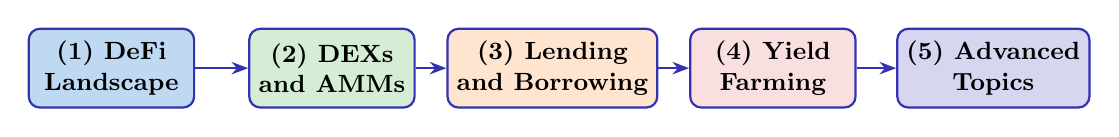
\begin{tikzpicture}[
    procstep/.style={rectangle, rounded corners=4pt, minimum width=2.1cm, minimum height=1.0cm,
      draw=mlpurple, thick, align=center, font=\small\bfseries}
  ]
    \node[procstep, fill=mlblue!25]   (b1) at (0,0)    {(1) DeFi\\Landscape};
    \node[procstep, fill=mlgreen!20]  (b2) at (2.8,0)  {(2) DEXs\\and AMMs};
    \node[procstep, fill=mlorange!20] (b3) at (5.6,0)  {(3) Lending\\and Borrowing};
    \node[procstep, fill=mlred!15]    (b4) at (8.4,0)  {(4) Yield\\Farming};
    \node[procstep, fill=mlpurple!20] (b5) at (11.2,0) {(5) Advanced\\Topics};
    \draw[-{Stealth[length=6pt]}, thick, mlpurple] (b1.east) -- (b2.west);
    \draw[-{Stealth[length=6pt]}, thick, mlpurple] (b2.east) -- (b3.west);
    \draw[-{Stealth[length=6pt]}, thick, mlpurple] (b3.east) -- (b4.west);
    \draw[-{Stealth[length=6pt]}, thick, mlpurple] (b4.east) -- (b5.west);
  \end{tikzpicture}

  \vspace{4mm}
  \begin{columns}[T]
    \begin{column}{0.48\textwidth}
      \begin{block}{Learning Objectives}
        \begin{itemize}\setlength\itemsep{1pt}
          \item Understand the DeFi ecosystem and its architecture
          \item Analyse Automated Market Maker (AMM) mathematics
          \item Model lending protocols and interest rate curves
          \item Quantify yield farming returns and impermanent loss
          \item Evaluate risks: smart contract, oracle, economic
        \end{itemize}
      \end{block}
    \end{column}
    \begin{column}{0.48\textwidth}
      \begin{block}{Prerequisites}
        \begin{itemize}\setlength\itemsep{1pt}
          \item Lessons 1--4: Blockchain, Ethereum, ERC-20, smart contracts
          \item Basic calculus and algebra
          \item Familiarity with Solidity interfaces
          \item Understanding of token standards and gas
        \end{itemize}
      \end{block}
    \end{column}
  \end{columns}
  \bottomnote{Duration: 90 minutes | 5 sections | \textasciitilde55 frames | Prerequisite: Lessons 1--4}
\end{frame}

% Frame 3: Table of Contents
\begin{frame}{Table of Contents}
  \tableofcontents
  \bottomnote{Navigate through 5 sections covering DeFi landscape to advanced topics}
\end{frame}

\begin{frame}{Learning Objectives}
By the end of this lecture, you will be able to:
\begin{enumerate}
\item \textbf{Explain} the DeFi stack and how composability enables ``money legos''
\item \textbf{Calculate} AMM prices, slippage, and impermanent loss using the constant product formula
\item \textbf{Analyze} lending protocol mechanics (collateralization ratios, liquidation, health factors)
\item \textbf{Compare} yield farming strategies and distinguish real yield from token emissions
\item \textbf{Evaluate} DeFi security risks including flash loan attacks and MEV extraction
\end{enumerate}
\bottomnote{Bloom's taxonomy levels: Remember $\rightarrow$ Understand $\rightarrow$ Apply $\rightarrow$ Analyze $\rightarrow$ Evaluate $\rightarrow$ Create}
\end{frame}

%% ============================================================
%% SECTION 1: DeFi Landscape
%% ============================================================

\section{DeFi Landscape}

% Frame 4: Section Divider
\begin{frame}
  \begin{beamercolorbox}[sep=12pt,center,rounded=true,shadow=true]{palette quaternary}
    {\Large\bfseries Section 1: DeFi Landscape}\\{}\vspace{6pt}
    {\normalsize Defining DeFi, its ecosystem, metrics, and risks}
  \end{beamercolorbox}
  \vspace{8mm}
  \begin{columns}[T]
    \begin{column}{0.48\textwidth}
      \begin{block}{What you will learn}
        \begin{itemize}\setlength\itemsep{2pt}
          \item Definition and properties of DeFi
          \item CeFi vs.\ DeFi architecture comparison
          \item Major protocol categories and their roles
          \item Key metrics: TVL, APY, utilisation rate
        \end{itemize}
      \end{block}
    \end{column}
    \begin{column}{0.48\textwidth}
      \begin{block}{Frames in this section}
        \begin{itemize}\setlength\itemsep{2pt}
          \item Frame 5 -- What is DeFi?
          \item Frame 6 -- CeFi vs.\ DeFi comparison
          \item Frame 7 -- DeFi ecosystem map
          \item Frames 8--14 -- Metrics, growth, risks
        \end{itemize}
      \end{block}
    \end{column}
  \end{columns}
  \bottomnote{Section 1 | Frames 4--14 | DeFi Landscape}
\end{frame}

% Frame 5: What is Decentralized Finance?
\begin{frame}{What is Decentralized Finance?}
  \begin{columns}[T]
    \begin{column}{0.50\textwidth}
      \begin{block}{Definition}
        \textbf{DeFi} (Decentralized Finance) refers to financial services and applications built on
        public blockchains --- primarily Ethereum --- that operate without centralised intermediaries
        such as banks, brokers, or exchanges.
      \end{block}
      \vspace{3mm}
      \begin{block}{Core Properties}
        \begin{itemize}\setlength\itemsep{2pt}
          \item \textbf{Permissionless} -- anyone with a wallet can participate
          \item \textbf{Trustless} -- rules enforced by code, not institutions
          \item \textbf{Transparent} -- all logic and state on-chain, auditable
          \item \textbf{Non-custodial} -- users retain control of private keys
          \item \textbf{Composable} -- protocols interoperate like ``money legos''
        \end{itemize}
      \end{block}
    \end{column}
    \begin{column}{0.46\textwidth}
      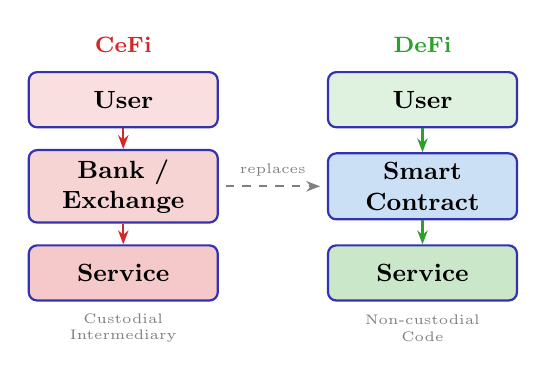
\begin{tikzpicture}[
        lbl/.style={rectangle, rounded corners=3pt, draw=mlpurple, thick,
                    minimum width=2.4cm, minimum height=0.7cm, align=center,
                    font=\small\bfseries},
        arr/.style={-{Stealth[length=5pt]}, thick}
      ]
        % CeFi column
        \node[lbl, fill=mlred!15]  (cu) at (0,3.2) {User};
        \node[lbl, fill=mlred!20]  (cb) at (0,2.1) {Bank /\\Exchange};
        \node[lbl, fill=mlred!25]  (cs) at (0,1.0) {Service};
        \draw[arr, mlred]   (cu.south) -- (cb.north);
        \draw[arr, mlred]   (cb.south) -- (cs.north);
        \node[font=\footnotesize\bfseries, mlred] at (0,3.9) {CeFi};
        \node[font=\tiny, mlgray, align=center] at (0,0.3) {Custodial\\Intermediary};

        % DeFi column
        \node[lbl, fill=mlgreen!15] (du) at (3.8,3.2) {User};
        \node[lbl, fill=mlblue!20]  (dc) at (3.8,2.1) {Smart\\Contract};
        \node[lbl, fill=mlgreen!25] (ds) at (3.8,1.0) {Service};
        \draw[arr, mlgreen] (du.south) -- (dc.north);
        \draw[arr, mlgreen] (dc.south) -- (ds.north);
        \node[font=\footnotesize\bfseries, mlgreen] at (3.8,3.9) {DeFi};
        \node[font=\tiny, mlgray, align=center] at (3.8,0.3) {Non-custodial\\Code};

        % Cross arrow
        \draw[arr, dashed, mlgray] (1.3,2.1) -- (2.5,2.1)
          node[midway, above, font=\tiny] {replaces};
      \end{tikzpicture}
    \end{column}
  \end{columns}
  \bottomnote{DeFi operates on public blockchains using smart contracts to replace traditional financial intermediaries}
\end{frame}

% Frame 6: CeFi vs DeFi Comparison
\begin{frame}{CeFi vs.\ DeFi: A Structural Comparison}
  \begin{columns}[T]
    \begin{column}{0.47\textwidth}
      \begin{block}{\textcolor{mlred}{Centralised Finance (CeFi)}}
        \begin{itemize}\setlength\itemsep{3pt}
          \item[\textcolor{mlred}{$\times$}] \textbf{Custody risk} -- exchange holds your assets
          \item[\textcolor{mlred}{$\times$}] \textbf{KYC/AML required} -- identity verification mandatory
          \item[\textcolor{mlred}{$\times$}] \textbf{Business hours} -- limited to operating times
          \item[\textcolor{mlred}{$\times$}] \textbf{Geographic restrictions} -- jurisdictional barriers
          \item[\textcolor{mlred}{$\times$}] \textbf{Opaque} -- internal risk not publicly visible
          \item[\textcolor{mlred}{$\times$}] \textbf{Censorship} -- accounts can be frozen
          \item[\textcolor{mlred}{$\times$}] \textbf{Single point of failure} -- operational risk
        \end{itemize}
      \end{block}
    \end{column}
    \begin{column}{0.47\textwidth}
      \begin{block}{\textcolor{mlgreen}{Decentralised Finance (DeFi)}}
        \begin{itemize}\setlength\itemsep{3pt}
          \item[\textcolor{mlgreen}{$\checkmark$}] \textbf{Self-custody} -- you hold your keys
          \item[\textcolor{mlgreen}{$\checkmark$}] \textbf{Permissionless} -- no identity required
          \item[\textcolor{mlgreen}{$\checkmark$}] \textbf{24/7 operation} -- always accessible
          \item[\textcolor{mlgreen}{$\checkmark$}] \textbf{Global access} -- no geographic limits
          \item[\textcolor{mlgreen}{$\checkmark$}] \textbf{Transparent} -- all logic on-chain, auditable
          \item[\textcolor{mlgreen}{$\checkmark$}] \textbf{Censorship-resistant} -- no authority to freeze
          \item[\textcolor{mlgreen}{$\checkmark$}] \textbf{Composable} -- interoperable protocols
        \end{itemize}
      \end{block}
    \end{column}
  \end{columns}
  \vspace{4mm}
  \begin{block}{Analogy}
    CeFi is like a traditional bank vault --- secure but gated. DeFi is like a vending machine ---
    rules are mechanical, visible, and execute automatically without a cashier.
  \end{block}
  \bottomnote{DeFi trades counterparty risk for smart contract risk; neither model is universally superior}
\end{frame}

% Frame 7: DeFi Ecosystem Map
\begin{frame}{DeFi Ecosystem Map}
  \centering
  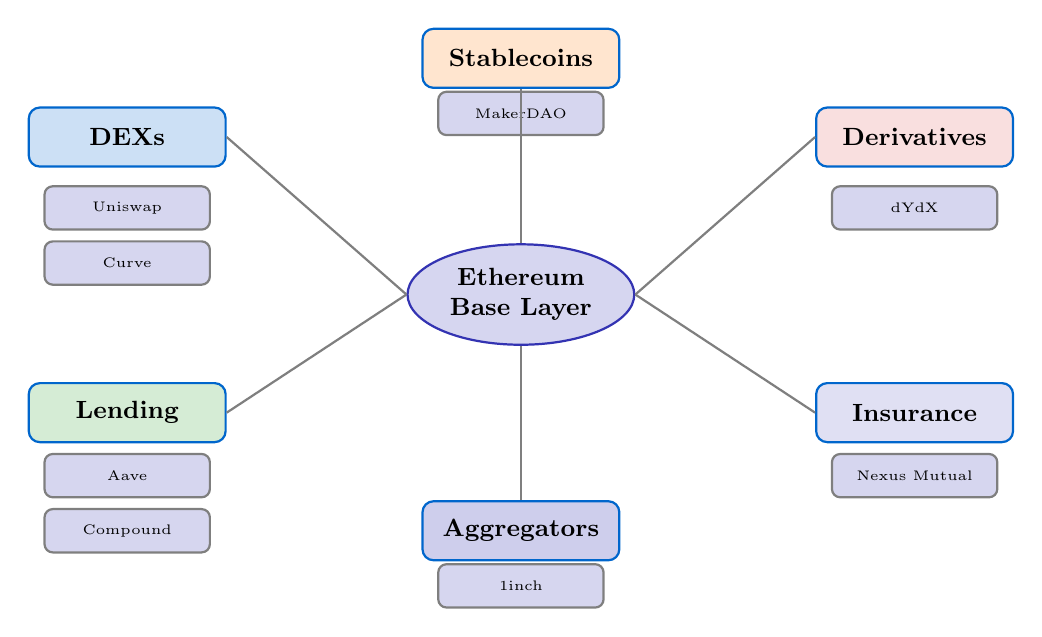
\begin{tikzpicture}[
    ctr/.style={ellipse, draw=mlpurple, fill=mlpurple!20, thick,
                minimum width=2.2cm, minimum height=1.0cm, align=center, font=\small\bfseries},
    cat/.style={rectangle, rounded corners=4pt, draw=mlblue, fill=mlblue!15, thick,
                minimum width=2.5cm, minimum height=0.75cm, align=center, font=\small\bfseries},
    sub/.style={rectangle, rounded corners=3pt, draw=mlgray, fill=mllavender4, thick,
                minimum width=2.1cm, minimum height=0.55cm, align=center, font=\tiny},
    conn/.style={thick, mlgray}
  ]
    % Centre
    \node[ctr] (eth) at (0,0) {Ethereum\\Base Layer};

    % DEXs
    \node[cat, fill=mlblue!20]    (dex)  at (-5.0, 2.0) {DEXs};
    \node[sub]                    (uni)  at (-5.0, 1.1) {Uniswap};
    \node[sub]                    (crv)  at (-5.0, 0.4) {Curve};

    % Lending
    \node[cat, fill=mlgreen!20]   (lend) at (-5.0,-1.5) {Lending};
    \node[sub]                    (aav)  at (-5.0,-2.3) {Aave};
    \node[sub]                    (cmp)  at (-5.0,-3.0) {Compound};

    % Stablecoins
    \node[cat, fill=mlorange!20]  (stbl) at (0.0, 3.0) {Stablecoins};
    \node[sub]                    (mkr)  at (0.0, 2.3) {MakerDAO};

    % Derivatives
    \node[cat, fill=mlred!15]     (derv) at (5.0, 2.0) {Derivatives};
    \node[sub]                    (dyd)  at (5.0, 1.1) {dYdX};

    % Insurance
    \node[cat, fill=mlpurple!15]  (ins)  at (5.0,-1.5) {Insurance};
    \node[sub]                    (nxs)  at (5.0,-2.3) {Nexus Mutual};

    % Aggregators
    \node[cat, fill=mllavender!60](agg)  at (0.0,-3.0) {Aggregators};
    \node[sub]                    (onei) at (0.0,-3.7) {1inch};

    % Connections
    \draw[conn] (eth.west)  -- (dex.east);
    \draw[conn] (eth.west)  -- (lend.east);
    \draw[conn] (eth.north) -- (stbl.south);
    \draw[conn] (eth.east)  -- (derv.west);
    \draw[conn] (eth.east)  -- (ins.west);
    \draw[conn] (eth.south) -- (agg.north);
  \end{tikzpicture}
  \bottomnote{Ethereum hosts the largest DeFi ecosystem; most protocols interact via standardised token interfaces}
\end{frame}

% Frame 8: Total Value Locked
\begin{frame}{Total Value Locked (TVL): The DeFi Thermometer}
  \begin{columns}[T]
    \begin{column}{0.52\textwidth}
      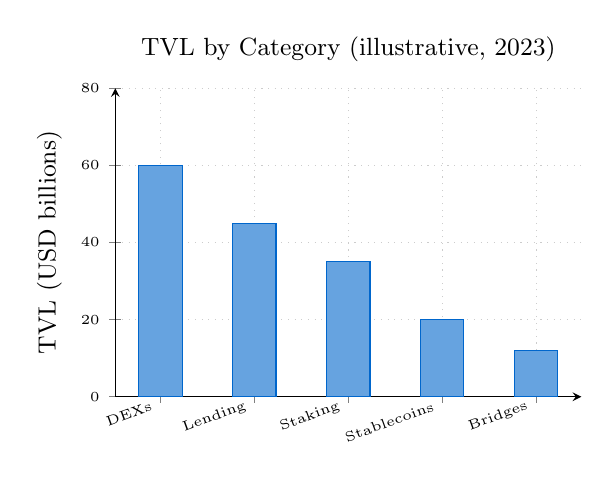
\begin{tikzpicture}
        \begin{axis}[
          width=7.5cm, height=5.5cm,
          ybar,
          bar width=0.55cm,
          symbolic x coords={DEXs, Lending, Staking, Stablecoins, Bridges},
          xtick=data,
          xticklabel style={font=\tiny, rotate=20, anchor=east},
          yticklabel style={font=\tiny},
          ylabel={\small TVL (USD billions)},
          ylabel style={font=\small},
          ymin=0, ymax=80,
          ytick={0,20,40,60,80},
          axis lines=left,
          enlarge x limits=0.12,
          grid=major,
          grid style={dotted, mlgray!40},
          title={\small TVL by Category (illustrative, 2023)},
          title style={font=\small},
        ]
          \addplot[fill=mlblue!60, draw=mlblue]
            coordinates {(DEXs,60) (Lending,45) (Staking,35) (Stablecoins,20) (Bridges,12)};
        \end{axis}
      \end{tikzpicture}
    \end{column}
    \begin{column}{0.44\textwidth}
      \begin{block}{TVL Definition}
        \[
          \mathrm{TVL} = \sum_{i=1}^{N} q_i \cdot p_i
        \]
        where $q_i$ is quantity of asset $i$ locked in protocol contracts and $p_i$ its USD price.
      \end{block}
      \vspace{3mm}
      \begin{block}{Limitations of TVL}
        \begin{itemize}\setlength\itemsep{2pt}
          \item \textbf{Double-counting}: same capital deposited in multiple layers
          \item \textbf{Price volatility}: TVL changes with asset prices, not just flows
          \item \textbf{Recursive leverage}: borrowed assets re-deposited inflate TVL
          \item \textbf{Not revenue}: high TVL $\neq$ high protocol earnings
        \end{itemize}
      \end{block}
    \end{column}
  \end{columns}
  \bottomnote{TVL is the most widely cited DeFi metric but must be interpreted alongside volume, fees, and protocol revenue}
\end{frame}

% Frame 9: DeFi Growth Timeline
\begin{frame}{DeFi Growth Timeline}
  \centering
  \adjustbox{max width=\textwidth}{%
  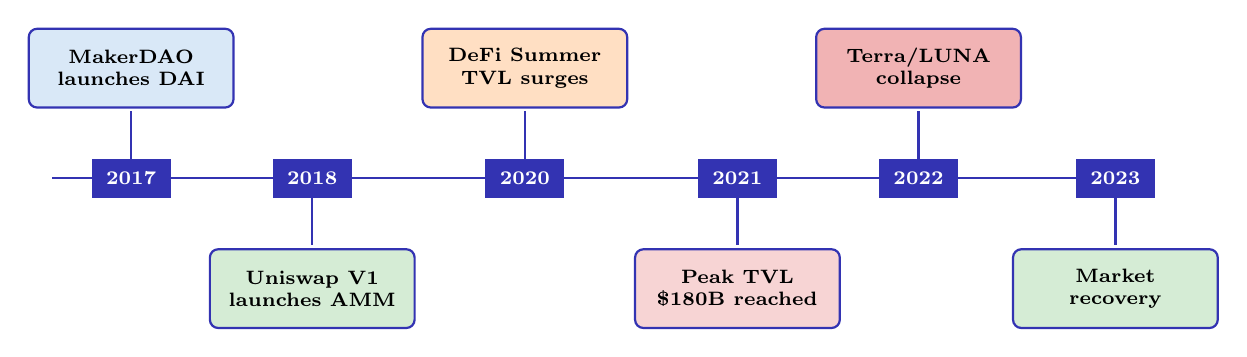
\begin{tikzpicture}[
    evtbox/.style={rectangle, rounded corners=3pt, draw=mlpurple, thick,
                   minimum width=2.6cm, minimum height=1.0cm, align=center,
                   font=\scriptsize\bfseries},
    datebox/.style={rectangle, fill=mlpurple, text=white,
                    minimum width=1.0cm, minimum height=0.5cm, align=center,
                    font=\scriptsize\bfseries}
  ]
    % Horizontal spine
    \draw[thick, mlpurple] (-0.5,0) -- (13.5,0);

    % Event 1: 2017 MakerDAO
    \node[datebox]  at (0.5,0)   {2017};
    \node[evtbox, fill=mlblue!15]   at (0.5, 1.4) {MakerDAO\\launches DAI};
    \draw[thick, mlpurple] (0.5,0.25) -- (0.5,0.85);

    % Event 2: 2018 Uniswap V1
    \node[datebox]  at (2.8,0)   {2018};
    \node[evtbox, fill=mlgreen!20]  at (2.8,-1.4) {Uniswap V1\\launches AMM};
    \draw[thick, mlpurple] (2.8,-0.25) -- (2.8,-0.85);

    % Event 3: 2020 DeFi Summer
    \node[datebox]  at (5.5,0)   {2020};
    \node[evtbox, fill=mlorange!25] at (5.5, 1.4) {DeFi Summer\\TVL surges};
    \draw[thick, mlpurple] (5.5,0.25) -- (5.5,0.85);

    % Event 4: 2021 Peak TVL
    \node[datebox]  at (8.2,0)   {2021};
    \node[evtbox, fill=mlred!20]    at (8.2,-1.4) {Peak TVL\\\$180B reached};
    \draw[thick, mlpurple] (8.2,-0.25) -- (8.2,-0.85);

    % Event 5: 2022 Terra collapse
    \node[datebox]  at (10.5,0)  {2022};
    \node[evtbox, fill=mlred!35]    at (10.5, 1.4) {Terra/LUNA\\collapse};
    \draw[thick, mlpurple] (10.5,0.25) -- (10.5,0.85);

    % Event 6: 2023 Recovery
    \node[datebox]  at (13.0,0)  {2023};
    \node[evtbox, fill=mlgreen!20]  at (13.0,-1.4) {Market\\recovery};
    \draw[thick, mlpurple] (13.0,-0.25) -- (13.0,-0.85);
  \end{tikzpicture}
  }%
  \bottomnote{DeFi grew from a single stablecoin protocol in 2017 to a multi-hundred-billion-dollar ecosystem by 2021}
\end{frame}

% Frame 10: Composability -- Money Legos
\begin{frame}{Composability: Money Legos}
  \begin{columns}[T]
    \begin{column}{0.52\textwidth}
      \centering
      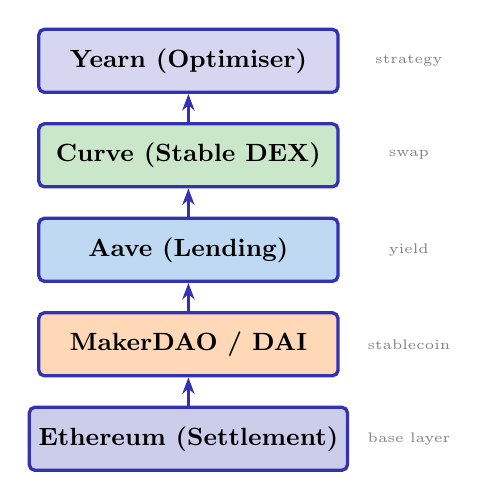
\begin{tikzpicture}[
        lego/.style={rectangle, rounded corners=2pt, draw=mlpurple, very thick,
                     minimum width=3.8cm, minimum height=0.8cm, align=center,
                     font=\small\bfseries},
        varr/.style={-{Stealth[length=6pt]}, thick, mlpurple}
      ]
        \node[lego, fill=mllavender3]  (eth)  at (0,0)   {Ethereum (Settlement)};
        \node[lego, fill=mlorange!30]  (dai)  at (0,1.2) {MakerDAO / DAI};
        \node[lego, fill=mlblue!25]    (aave) at (0,2.4) {Aave (Lending)};
        \node[lego, fill=mlgreen!25]   (crv)  at (0,3.6) {Curve (Stable DEX)};
        \node[lego, fill=mlpurple!20]  (yearn)at (0,4.8) {Yearn (Optimiser)};

        \draw[varr] (eth.north)  -- (dai.south);
        \draw[varr] (dai.north)  -- (aave.south);
        \draw[varr] (aave.north) -- (crv.south);
        \draw[varr] (crv.north)  -- (yearn.south);

        \node[font=\tiny, mlgray] at (2.8,0)   {base layer};
        \node[font=\tiny, mlgray] at (2.8,1.2) {stablecoin};
        \node[font=\tiny, mlgray] at (2.8,2.4) {yield};
        \node[font=\tiny, mlgray] at (2.8,3.6) {swap};
        \node[font=\tiny, mlgray] at (2.8,4.8) {strategy};
      \end{tikzpicture}
    \end{column}
    \begin{column}{0.44\textwidth}
      \begin{block}{What is Composability?}
        DeFi protocols expose standardised interfaces (ERC-20, ERC-4626) that allow any protocol to
        build on top of another without permission. One transaction can:
        \begin{enumerate}\setlength\itemsep{2pt}
          \item Borrow DAI from Aave
          \item Swap DAI for USDC on Curve
          \item Deposit USDC into Yearn vault
          \item Receive yield-bearing tokens
        \end{enumerate}
        --- all atomically, in a single call.
      \end{block}
      \vspace{3mm}
      \begin{alertblock}{Systemic Risk}
        Composability also propagates failures: a bug in one protocol can cascade through all
        protocols that depend on it --- analogous to a shared library vulnerability.
      \end{alertblock}
    \end{column}
  \end{columns}
  \bottomnote{Composability is DeFi's greatest strength and its most significant systemic risk vector}
\end{frame}

% Frame 11: Key DeFi Metrics
\begin{frame}{Key DeFi Metrics}
  \centering
  \adjustbox{max width=\textwidth}{%
  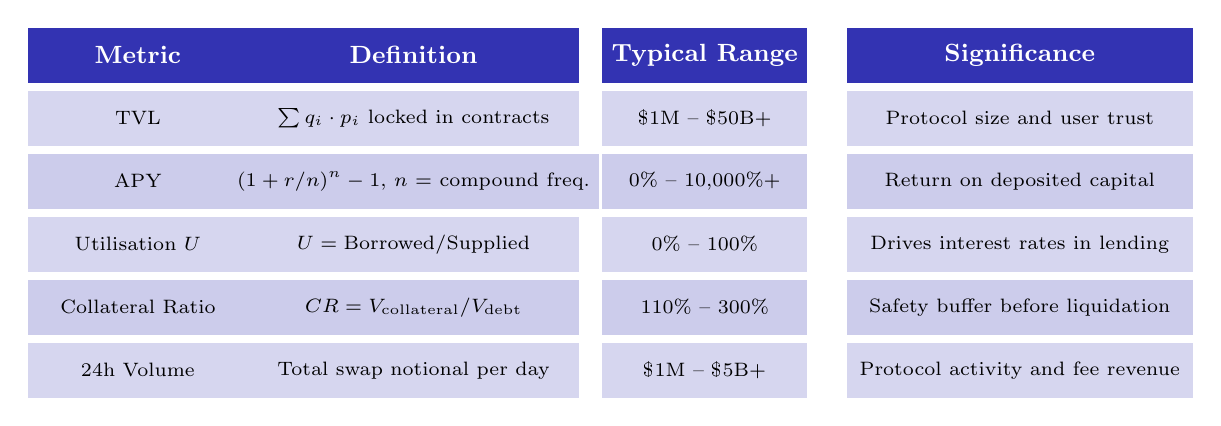
\begin{tikzpicture}[
    hdr/.style={rectangle, fill=mlpurple, text=white, minimum height=0.7cm,
                align=center, font=\small\bfseries},
    cel/.style={rectangle, fill=mllavender4, minimum height=0.7cm,
                align=center, font=\scriptsize},
    altcel/.style={rectangle, fill=mllavender3, minimum height=0.7cm,
                   align=center, font=\scriptsize}
  ]
    % Header row
    \node[hdr, minimum width=2.8cm] (h1) at (0,0)    {Metric};
    \node[hdr, minimum width=4.2cm] (h2) at (3.5,0)  {Definition};
    \node[hdr, minimum width=2.6cm] (h3) at (7.2,0)  {Typical Range};
    \node[hdr, minimum width=4.4cm] (h4) at (11.2,0) {Significance};

    % Row 1: TVL
    \node[cel, minimum width=2.8cm] at (0,-0.8)    {TVL};
    \node[cel, minimum width=4.2cm, align=left] at (3.5,-0.8)
      {$\sum q_i \cdot p_i$ locked in contracts};
    \node[cel, minimum width=2.6cm] at (7.2,-0.8)  {\$1M -- \$50B+};
    \node[cel, minimum width=4.4cm, align=left] at (11.2,-0.8)
      {Protocol size and user trust};

    % Row 2: APY
    \node[altcel, minimum width=2.8cm] at (0,-1.6)   {APY};
    \node[altcel, minimum width=4.2cm, align=left] at (3.5,-1.6)
      {$(1 + r/n)^n - 1$, $n$ = compound freq.};
    \node[altcel, minimum width=2.6cm] at (7.2,-1.6) {0\% -- 10,000\%+};
    \node[altcel, minimum width=4.4cm, align=left] at (11.2,-1.6)
      {Return on deposited capital};

    % Row 3: Utilisation Rate
    \node[cel, minimum width=2.8cm] at (0,-2.4)    {Utilisation $U$};
    \node[cel, minimum width=4.2cm, align=left] at (3.5,-2.4)
      {$U = \text{Borrowed} / \text{Supplied}$};
    \node[cel, minimum width=2.6cm] at (7.2,-2.4)  {0\% -- 100\%};
    \node[cel, minimum width=4.4cm, align=left] at (11.2,-2.4)
      {Drives interest rates in lending};

    % Row 4: Collateral Ratio
    \node[altcel, minimum width=2.8cm] at (0,-3.2)   {Collateral Ratio};
    \node[altcel, minimum width=4.2cm, align=left] at (3.5,-3.2)
      {$CR = V_{\text{collateral}} / V_{\text{debt}}$};
    \node[altcel, minimum width=2.6cm] at (7.2,-3.2) {110\% -- 300\%};
    \node[altcel, minimum width=4.4cm, align=left] at (11.2,-3.2)
      {Safety buffer before liquidation};

    % Row 5: Volume
    \node[cel, minimum width=2.8cm] at (0,-4.0)    {24h Volume};
    \node[cel, minimum width=4.2cm, align=left] at (3.5,-4.0)
      {Total swap notional per day};
    \node[cel, minimum width=2.6cm] at (7.2,-4.0)  {\$1M -- \$5B+};
    \node[cel, minimum width=4.4cm, align=left] at (11.2,-4.0)
      {Protocol activity and fee revenue};
  \end{tikzpicture}
  }%
  \bottomnote{Metrics should be evaluated together; a high APY with low TVL and high utilisation may signal unsustainable incentives}
\end{frame}

% Frame 12: DeFi Risks Overview
\begin{frame}{DeFi Risks Overview}
  \begin{columns}[T]
    \begin{column}{0.47\textwidth}
      \begin{block}{Technical Risks}
        \begin{itemize}\setlength\itemsep{3pt}
          \item \textbf{Smart contract bugs} -- reentrancy, overflow, access control
          \item \textbf{Oracle manipulation} -- price feed attacks, flash loan exploits
          \item \textbf{Bridge vulnerabilities} -- cross-chain message forgery
          \item \textbf{MEV / front-running} -- sandwich attacks on AMM trades
          \item \textbf{Upgradeability risk} -- admin key compromise, proxy hijacking
        \end{itemize}
      \end{block}
    \end{column}
    \begin{column}{0.47\textwidth}
      \begin{block}{Economic Risks}
        \begin{itemize}\setlength\itemsep{3pt}
          \item \textbf{Impermanent loss} -- AMM LPs lose vs.\ holding during volatility
          \item \textbf{Liquidation cascades} -- falling prices trigger mass liquidations
          \item \textbf{Stablecoin depeg} -- collateral or peg mechanism failure
          \item \textbf{Governance attacks} -- token accumulation to pass malicious proposals
          \item \textbf{Unsustainable yields} -- token emission Ponzis, yield collapse
        \end{itemize}
      \end{block}
    \end{column}
  \end{columns}
  \vspace{4mm}
  \begin{alertblock}{Warning: DeFi is Experimental Software}
    Over \$5 billion has been lost to DeFi exploits since 2020. Users must conduct independent risk
    assessment before interacting with any protocol, regardless of audit status or TVL.
  \end{alertblock}
  \bottomnote{Risk management in DeFi requires simultaneous assessment of technical, economic, and governance dimensions}
\end{frame}

% Frame 13: Major DeFi Hacks
\begin{frame}{Major DeFi Hacks: A Security Retrospective}
  \centering
  \adjustbox{max width=\textwidth}{%
  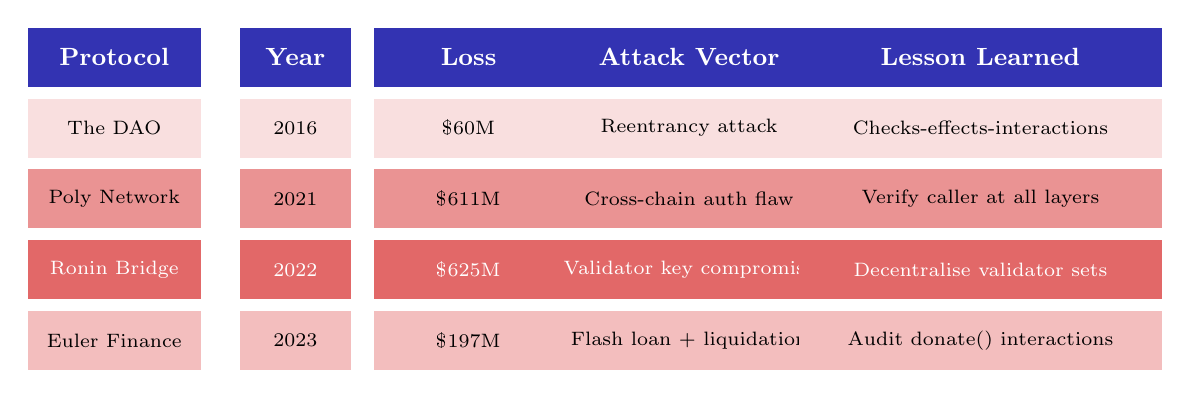
\begin{tikzpicture}[
    hdr/.style={rectangle, minimum height=0.75cm, align=center,
                font=\small\bfseries, text=white},
    sev1/.style={rectangle, minimum height=0.75cm, align=center,
                 font=\scriptsize, fill=mlred!15},
    sev2/.style={rectangle, minimum height=0.75cm, align=center,
                 font=\scriptsize, fill=mlred!30},
    sev3/.style={rectangle, minimum height=0.75cm, align=center,
                 font=\scriptsize, fill=mlred!50},
    sev4/.style={rectangle, minimum height=0.75cm, align=center,
                 font=\scriptsize, fill=mlred!70, text=white}
  ]
    % Header
    \node[hdr, minimum width=2.2cm, fill=mlpurple]   at (0,0)     {Protocol};
    \node[hdr, minimum width=1.4cm, fill=mlpurple]   at (2.3,0)   {Year};
    \node[hdr, minimum width=2.4cm, fill=mlpurple]   at (4.5,0)   {Loss};
    \node[hdr, minimum width=3.6cm, fill=mlpurple]   at (7.3,0)   {Attack Vector};
    \node[hdr, minimum width=4.6cm, fill=mlpurple]   at (11.0,0)  {Lesson Learned};

    % Row 1: The DAO
    \node[sev1, minimum width=2.2cm] at (0,-0.9)    {The DAO};
    \node[sev1, minimum width=1.4cm] at (2.3,-0.9)  {2016};
    \node[sev1, minimum width=2.4cm] at (4.5,-0.9)  {\$60M};
    \node[sev1, minimum width=3.6cm] at (7.3,-0.9)  {Reentrancy attack};
    \node[sev1, minimum width=4.6cm] at (11.0,-0.9) {Checks-effects-interactions};

    % Row 2: Poly Network
    \node[sev3, minimum width=2.2cm] at (0,-1.8)    {Poly Network};
    \node[sev3, minimum width=1.4cm] at (2.3,-1.8)  {2021};
    \node[sev3, minimum width=2.4cm] at (4.5,-1.8)  {\$611M};
    \node[sev3, minimum width=3.6cm] at (7.3,-1.8)  {Cross-chain auth flaw};
    \node[sev3, minimum width=4.6cm] at (11.0,-1.8) {Verify caller at all layers};

    % Row 3: Ronin Bridge
    \node[sev4, minimum width=2.2cm] at (0,-2.7)    {Ronin Bridge};
    \node[sev4, minimum width=1.4cm] at (2.3,-2.7)  {2022};
    \node[sev4, minimum width=2.4cm] at (4.5,-2.7)  {\$625M};
    \node[sev4, minimum width=3.6cm] at (7.3,-2.7)  {Validator key compromise};
    \node[sev4, minimum width=4.6cm] at (11.0,-2.7) {Decentralise validator sets};

    % Row 4: Euler Finance
    \node[sev2, minimum width=2.2cm] at (0,-3.6)    {Euler Finance};
    \node[sev2, minimum width=1.4cm] at (2.3,-3.6)  {2023};
    \node[sev2, minimum width=2.4cm] at (4.5,-3.6)  {\$197M};
    \node[sev2, minimum width=3.6cm] at (7.3,-3.6)  {Flash loan + liquidation};
    \node[sev2, minimum width=4.6cm] at (11.0,-3.6) {Audit donate() interactions};
  \end{tikzpicture}
  }%

  \vspace{3mm}
  \footnotesize\textit{Note: Ronin Bridge funds were partially returned; Euler attacker returned most funds.}
  \bottomnote{The largest hacks exploited logic flaws, not brute-force cryptography; audits reduce but do not eliminate risk}
\end{frame}

% Frame 14: Section 1 Summary
\begin{frame}{Section 1 Summary: DeFi Landscape}
  \begin{columns}[T]
    \begin{column}{0.48\textwidth}
      \begin{block}{Key Takeaways}
        \begin{itemize}\setlength\itemsep{4pt}
          \item \textbf{DeFi} replaces intermediaries with smart contracts, enabling permissionless,
                transparent, and composable financial services
          \item \textbf{TVL, APY, and utilisation rate} are the primary metrics --- each with
                important caveats and limitations
          \item \textbf{Composability} (``money legos'') unlocks novel financial primitives but
                introduces systemic contagion risk
          \item \textbf{Technical and economic risks} are both significant; over \$5B lost to
                exploits since 2020
          \item \textbf{DeFi growth} from MakerDAO (2017) to \$180B TVL peak (2021) demonstrated
                product-market fit despite volatility
        \end{itemize}
      \end{block}
    \end{column}
    \begin{column}{0.48\textwidth}
      \begin{block}{Formulas to Remember}
        \[
          \mathrm{TVL} = \sum_{i} q_i \cdot p_i
        \]
        \[
          \mathrm{APY} = \left(1 + \frac{r}{n}\right)^n - 1
        \]
        \[
          U = \frac{\text{Total Borrowed}}{\text{Total Supplied}}
        \]
        \[
          CR = \frac{V_{\text{collateral}}}{V_{\text{debt}}} \geq CR_{\min}
        \]
      \end{block}
      \vspace{3mm}
      \begin{alertblock}{Coming Up: Section 2}
        DEXs and Automated Market Makers --- the mathematical engine behind decentralised trading.
      \end{alertblock}
    \end{column}
  \end{columns}
  \bottomnote{Section 1 complete | Next: Section 2 --- DEXs and AMMs | Frames 15 onward}
\end{frame}

%% ============================================================
%% SECTION 2: DEXs and AMMs
%% ============================================================

\section{DEXs \& Automated Market Makers}

% Frame 15: Section Divider
\begin{frame}
  \begin{beamercolorbox}[sep=12pt,center,rounded=true,shadow=true]{palette quaternary}
    {\Large\bfseries Section 2: DEXs and Automated Market Makers}\\{}\vspace{6pt}
    {\normalsize Constant product formula, price impact, slippage, LP mechanics, and impermanent loss}
  \end{beamercolorbox}
  \vspace{8mm}
  \begin{columns}[T]
    \begin{column}{0.48\textwidth}
      \begin{block}{What you will learn}
        \begin{itemize}\setlength\itemsep{2pt}
          \item Order books vs.\ AMM pool architecture
          \item Constant product formula $x \cdot y = k$ and its geometry
          \item Price impact, slippage, and execution cost
          \item Liquidity provision mechanics and fee accrual
          \item Impermanent loss derivation and mitigation
        \end{itemize}
      \end{block}
    \end{column}
    \begin{column}{0.48\textwidth}
      \begin{block}{Frames in this section}
        \begin{itemize}\setlength\itemsep{2pt}
          \item Frame 16 -- Order Books vs.\ AMMs
          \item Frame 17 -- The Constant Product Formula
          \item Frames 18--19 -- Worked example, price impact
          \item Frames 20--21 -- Slippage, LP mechanics
          \item Frames 22--26 -- Uniswap V3, AMM models, IL, aggregators
        \end{itemize}
      \end{block}
    \end{column}
  \end{columns}
  \bottomnote{Section 2 | Frames 15--26 | DEXs and Automated Market Makers}
\end{frame}

% Frame 16: Order Books vs AMMs
\begin{frame}{Order Books vs.\ AMMs}
  \begin{columns}[T]
    \begin{column}{0.46\textwidth}
      \centering
      \textbf{\textcolor{mlblue}{Order Book (CeFi/CEX)}}
      \vspace{3mm}

      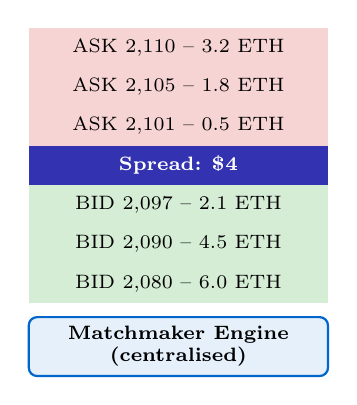
\begin{tikzpicture}[
        bidrow/.style={rectangle, fill=mlgreen!20, minimum width=3.8cm,
                       minimum height=0.5cm, align=center, font=\scriptsize},
        askrow/.style={rectangle, fill=mlred!20,  minimum width=3.8cm,
                       minimum height=0.5cm, align=center, font=\scriptsize},
        midlbl/.style={rectangle, fill=mlpurple,  minimum width=3.8cm,
                       minimum height=0.5cm, align=center, font=\scriptsize\bfseries, text=white},
        mmbox/.style={rectangle, rounded corners=3pt, draw=mlblue, thick,
                      minimum width=3.8cm, minimum height=0.7cm, align=center, font=\scriptsize\bfseries}
      ]
        \node[askrow] at (0, 2.2) {ASK 2,110 -- 3.2 ETH};
        \node[askrow] at (0, 1.7) {ASK 2,105 -- 1.8 ETH};
        \node[askrow] at (0, 1.2) {ASK 2,101 -- 0.5 ETH};
        \node[midlbl] at (0, 0.7) {Spread: \$4};
        \node[bidrow] at (0, 0.2) {BID 2,097 -- 2.1 ETH};
        \node[bidrow] at (0,-0.3) {BID 2,090 -- 4.5 ETH};
        \node[bidrow] at (0,-0.8) {BID 2,080 -- 6.0 ETH};
        \node[mmbox, fill=mlblue!10] at (0,-1.6) {Matchmaker Engine\\(centralised)};
      \end{tikzpicture}
    \end{column}
    \begin{column}{0.46\textwidth}
      \centering
      \textbf{\textcolor{mlgreen}{AMM Pool (DeFi/DEX)}}
      \vspace{3mm}

      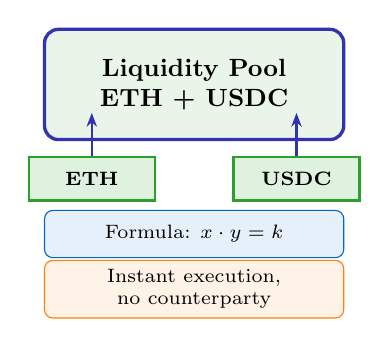
\begin{tikzpicture}[
        poolbox/.style={rectangle, rounded corners=5pt, draw=mlpurple, very thick,
                        minimum width=3.8cm, minimum height=1.4cm, align=center,
                        font=\small\bfseries},
        lblbox/.style={rectangle, fill=mlgreen!15, draw=mlgreen, thick,
                       minimum width=1.6cm, minimum height=0.55cm, align=center,
                       font=\scriptsize\bfseries},
        fmla/.style={rectangle, fill=mlblue!10, draw=mlblue, rounded corners=3pt,
                     minimum width=3.8cm, minimum height=0.6cm, align=center,
                     font=\scriptsize}
      ]
        \node[poolbox, fill=mlgreen!10] (pool) at (0,1.2) {Liquidity Pool\\ETH + USDC};
        \node[lblbox] (tok1) at (-1.3, 0.0) {ETH};
        \node[lblbox] (tok2) at ( 1.3, 0.0) {USDC};
        \draw[-{Stealth[length=5pt]}, thick, mlpurple] (tok1.north) -- ++(0,0.55);
        \draw[-{Stealth[length=5pt]}, thick, mlpurple] (tok2.north) -- ++(0,0.55);
        \node[fmla] at (0,-0.7) {Formula: $x \cdot y = k$};
        \node[fmla, fill=mlorange!10, draw=mlorange] at (0,-1.4) {Instant execution,\\no counterparty};
      \end{tikzpicture}
    \end{column}
  \end{columns}
  \vspace{3mm}
  \begin{center}
  \footnotesize
  \begin{tabular}{lll}
    \toprule
    \textbf{Property} & \textbf{Order Book} & \textbf{AMM} \\
    \midrule
    Price discovery  & Bid/ask matching      & Formula-determined \\
    Liquidity        & Maker orders          & Pooled reserves     \\
    Execution speed  & Depends on liquidity  & Instant             \\
    Counterparty     & Another trader        & The pool contract   \\
    Capital eff.     & High (concentrated)   & Low (full range)    \\
    \bottomrule
  \end{tabular}
  \end{center}
  \bottomnote{AMMs replace discrete order matching with a continuous pricing function; liquidity providers replace market makers}
\end{frame}

% Frame 17: The Constant Product Formula
\begin{frame}{The Constant Product Formula}
  \begin{columns}[T]
    \begin{column}{0.50\textwidth}
      \vspace{2mm}
      \begin{block}{Core Invariant}
        \[
          x \cdot y = k
        \]
        where $x$ = reserve of token X, $y$ = reserve of token Y, $k$ = constant (invariant).
      \end{block}
      \vspace{3mm}
      \begin{block}{Step-by-Step Derivation}
        \begin{enumerate}\setlength\itemsep{3pt}
          \item Initial state: $x_0 \cdot y_0 = k$
          \item Trader sends $\Delta x$ of token X to pool
          \item New reserve: $x_1 = x_0 + \Delta x$
          \item Invariant must hold: $x_1 \cdot y_1 = k$
          \item Amount out: $\Delta y = y_0 - \dfrac{k}{x_0 + \Delta x}$
          \item Marginal price: $P = \dfrac{y_0}{x_0}$ (before trade)
          \item Effective price: $P_{\text{eff}} = \dfrac{\Delta y}{\Delta x}$
        \end{enumerate}
      \end{block}
    \end{column}
    \begin{column}{0.46\textwidth}
      \centering
      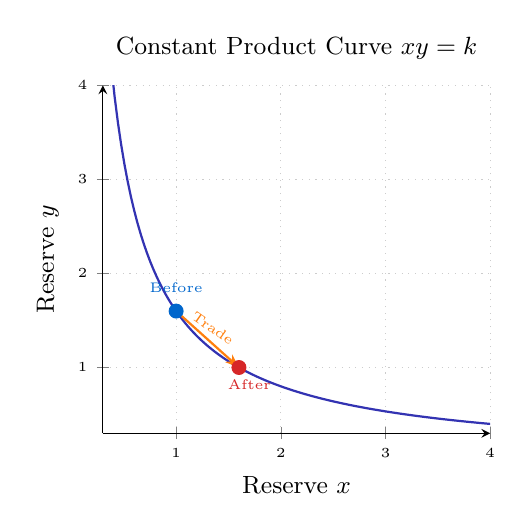
\begin{tikzpicture}
        \begin{axis}[
          width=6.5cm, height=6.0cm,
          xmin=0.3, xmax=4.0,
          ymin=0.3, ymax=4.0,
          xlabel={Reserve $x$},
          ylabel={Reserve $y$},
          xlabel style={font=\small},
          ylabel style={font=\small},
          xticklabel style={font=\tiny},
          yticklabel style={font=\tiny},
          axis lines=left,
          grid=major,
          grid style={dotted, mlgray!40},
          title={\small Constant Product Curve $xy=k$},
          title style={font=\small},
        ]
          \addplot[thick, mlpurple, domain=0.32:4.0, samples=120] {1.6/x};
          \addplot[only marks, mark=*, mark options={fill=mlblue, draw=mlblue}, mark size=2.5pt]
            coordinates {(1.0, 1.6)};
          \addplot[only marks, mark=*, mark options={fill=mlred, draw=mlred}, mark size=2.5pt]
            coordinates {(1.6, 1.0)};
          \addplot[-{Stealth[length=5pt]}, thick, mlorange]
            coordinates {(1.0,1.6) (1.6,1.0)};
          \node[font=\tiny, mlblue]  at (axis cs:1.0, 1.85) {Before};
          \node[font=\tiny, mlred]   at (axis cs:1.7, 0.82) {After};
          \node[font=\tiny, mlorange, rotate=-35] at (axis cs:1.35,1.42) {Trade};
        \end{axis}
      \end{tikzpicture}
    \end{column}
  \end{columns}
  \bottomnote{The constant product invariant ensures the pool always has reserves for any trade; only the price changes, never to zero}
\end{frame}

% Frame 18: Constant Product Worked Example
\begin{frame}{Constant Product: Worked Example}
  \begin{columns}[T]
    \begin{column}{0.48\textwidth}
      \begin{block}{Scenario: Buy 5 ETH from Pool}
        \begin{enumerate}\setlength\itemsep{4pt}
          \item \textbf{Initial pool}: 100 ETH + 200{,}000 USDC
          \item \textbf{Invariant}: $k = 100 \times 200{,}000 = 20{,}000{,}000$
          \item \textbf{Buy 5 ETH}: new ETH reserve $= 100 - 5 = 95$
          \item \textbf{New USDC reserve}:
                \[ y_1 = \frac{k}{x_1} = \frac{20{,}000{,}000}{95} \approx 210{,}526.32 \]
          \item \textbf{USDC cost}: $210{,}526.32 - 200{,}000 = \mathbf{10{,}526.32}$
          \item \textbf{Effective price}: $10{,}526.32 / 5 = \mathbf{\$2{,}105.26}$
          \item \textbf{Spot price before}: $200{,}000 / 100 = \$2{,}000.00$
          \item \textbf{Price impact}: $(2105.26 - 2000)/2000 = \mathbf{5.26\%}$
        \end{enumerate}
      \end{block}
    \end{column}
    \begin{column}{0.48\textwidth}
      \centering
      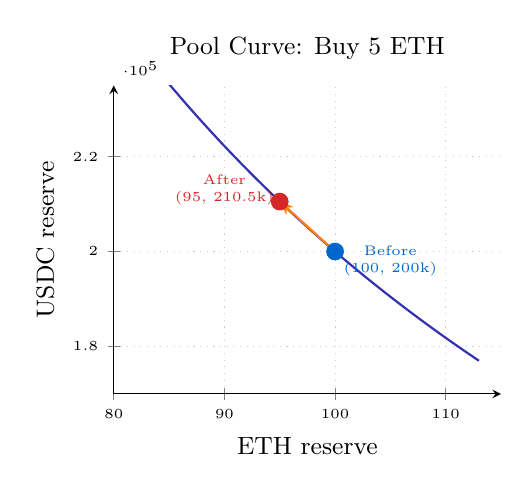
\begin{tikzpicture}
        \begin{axis}[
          width=6.5cm, height=5.5cm,
          xmin=80, xmax=115,
          ymin=170000, ymax=235000,
          xlabel={ETH reserve},
          ylabel={USDC reserve},
          xlabel style={font=\small},
          ylabel style={font=\small},
          xticklabel style={font=\tiny},
          yticklabel style={font=\tiny},
          axis lines=left,
          grid=major,
          grid style={dotted, mlgray!40},
          title={\small Pool Curve: Buy 5 ETH},
          title style={font=\small},
        ]
          \addplot[thick, mlpurple, domain=82:113, samples=100] {20000000/x};
          \addplot[only marks, mark=*, mark options={fill=mlblue, draw=mlblue}, mark size=3pt]
            coordinates {(100, 200000)};
          \addplot[only marks, mark=*, mark options={fill=mlred, draw=mlred}, mark size=3pt]
            coordinates {(95, 210526.32)};
          \addplot[-{Stealth[length=5pt]}, thick, mlorange]
            coordinates {(100,200000) (95,210526.32)};
          \node[font=\tiny, mlblue,  align=center] at (axis cs:105, 198000) {Before\\(100, 200k)};
          \node[font=\tiny, mlred,   align=center] at (axis cs:90,  213000) {After\\(95, 210.5k)};
        \end{axis}
      \end{tikzpicture}
    \end{column}
  \end{columns}
  \bottomnote{Price impact of 5.26\% arises from buying 5\% of the ETH reserve; larger trades relative to pool size incur more slippage}
\end{frame}

% Frame 19: Price Impact Visualization
\begin{frame}{Price Impact vs.\ Trade Size}
  \centering
  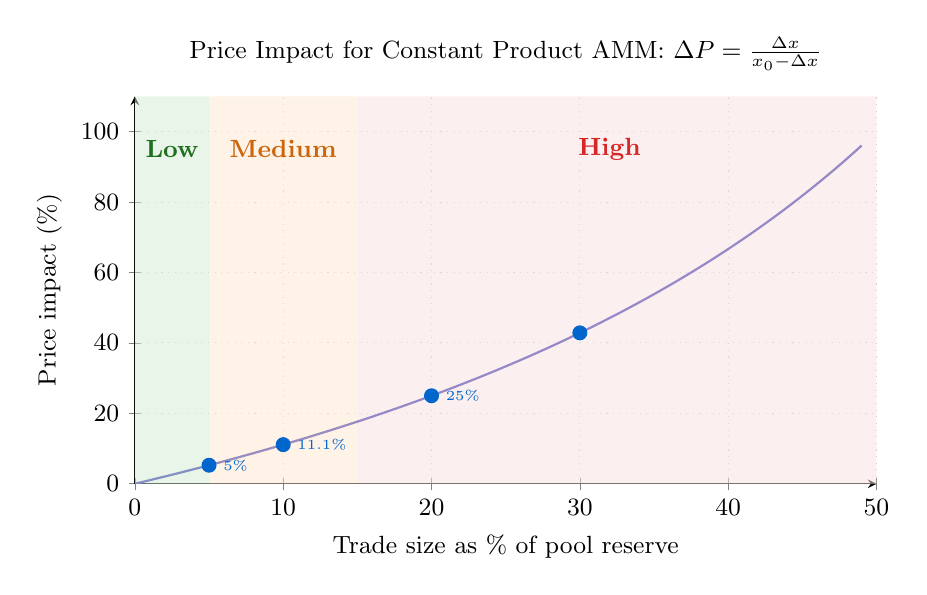
\begin{tikzpicture}
    \begin{axis}[
      width=11cm, height=6.5cm,
      xmin=0, xmax=50,
      ymin=0, ymax=110,
      xlabel={Trade size as \% of pool reserve},
      ylabel={Price impact (\%)},
      xlabel style={font=\small},
      ylabel style={font=\small},
      xticklabel style={font=\small},
      yticklabel style={font=\small},
      axis lines=left,
      grid=major,
      grid style={dotted, mlgray!40},
      title={\small Price Impact for Constant Product AMM: $\Delta P = \frac{\Delta x}{x_0 - \Delta x}$},
      title style={font=\small},
      xtick={0,10,20,30,40,50},
      ytick={0,20,40,60,80,100},
    ]
      % Price impact = delta_x / (x0 - delta_x) * 100
      % Let s = trade_size_pct / 100, then impact = s/(1-s)*100
      \addplot[thick, mlpurple, domain=0:49, samples=200] {(x/100)/(1-x/100)*100};
      % Green zone: 0-5%
      \addplot[fill=mlgreen!20, draw=none, opacity=0.5]
        coordinates {(0,0) (5,0) (5,110) (0,110)} \closedcycle;
      % Orange zone: 5-15%
      \addplot[fill=mlorange!20, draw=none, opacity=0.5]
        coordinates {(5,0) (15,0) (15,110) (5,110)} \closedcycle;
      % Red zone: 15-50%
      \addplot[fill=mlred!15, draw=none, opacity=0.5]
        coordinates {(15,0) (50,0) (50,110) (15,110)} \closedcycle;
      \node[font=\small\bfseries, mlgreen!70!black]  at (axis cs:2.5, 95) {Low};
      \node[font=\small\bfseries, mlorange!80!black] at (axis cs:10,  95) {Medium};
      \node[font=\small\bfseries, mlred]             at (axis cs:32,  95) {High};
      % Key point annotations
      \addplot[only marks, mark=*, mark options={fill=mlblue, draw=mlblue}, mark size=2.5pt]
        coordinates {(5, 5.26) (10, 11.11) (20, 25.0) (30, 42.86)};
      \node[font=\tiny, mlblue, anchor=west] at (axis cs:5.3, 5.26) {5\%};
      \node[font=\tiny, mlblue, anchor=west] at (axis cs:10.3, 11.11) {11.1\%};
      \node[font=\tiny, mlblue, anchor=west] at (axis cs:20.3, 25.0) {25\%};
    \end{axis}
  \end{tikzpicture}
  \bottomnote{Price impact grows super-linearly; trades $>$15\% of pool reserves are economically inadvisable without aggregation}
\end{frame}

% Frame 20: Slippage Explained
\begin{frame}{Slippage: Expected vs.\ Actual Price}
  \begin{columns}[T]
    \begin{column}{0.52\textwidth}
      \centering
      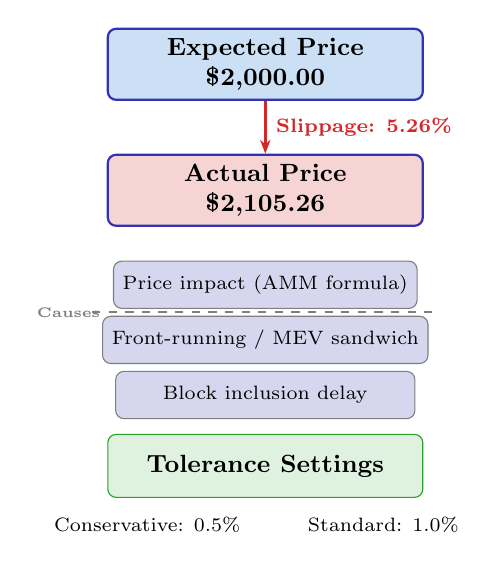
\begin{tikzpicture}[
        pricebox/.style={rectangle, rounded corners=3pt, draw=mlpurple, thick,
                         minimum width=4.0cm, minimum height=0.7cm, align=center,
                         font=\small\bfseries},
        causebox/.style={rectangle, rounded corners=3pt, draw=mlgray, fill=mllavender4,
                         minimum width=3.8cm, minimum height=0.6cm, align=center,
                         font=\scriptsize},
        arr/.style={-{Stealth[length=5pt]}, thick}
      ]
        \node[pricebox, fill=mlblue!20]   (exp) at (0,3.2) {Expected Price\\\$2,000.00};
        \node[pricebox, fill=mlred!20]    (act) at (0,1.6) {Actual Price\\\$2,105.26};
        \draw[arr, mlred, very thick]     (exp.south) -- (act.north)
          node[midway, right, font=\scriptsize\bfseries, mlred] {Slippage: 5.26\%};

        \node[causebox] (c1) at (0, 0.4) {Price impact (AMM formula)};
        \node[causebox] (c2) at (0,-0.3) {Front-running / MEV sandwich};
        \node[causebox] (c3) at (0,-1.0) {Block inclusion delay};

        \node[rectangle, fill=mlgreen!15, draw=mlgreen, rounded corners=3pt,
              minimum width=4.0cm, minimum height=0.8cm, align=center,
              font=\small\bfseries] at (0,-1.9) {Tolerance Settings};
        \node[font=\scriptsize] at (-1.5,-2.65) {Conservative: 0.5\%};
        \node[font=\scriptsize] at ( 1.5,-2.65) {Standard: 1.0\%};

        \node[font=\tiny, mlgray, align=center] at (0,0.0) {};
        \draw[thick, mlgray, dashed] (-2.2, 0.05) -- (2.2, 0.05)
          node[above, font=\tiny, mlgray] {};
        \node[font=\tiny\bfseries, mlgray] at (-2.5, 0.05) {Causes};
      \end{tikzpicture}
    \end{column}
    \begin{column}{0.44\textwidth}
      \begin{block}{Slippage Definition}
        \textbf{Slippage} is the difference between the price quoted at trade initiation and the
        price at which the trade actually executes on-chain.
        \[
          \text{Slippage} = \frac{P_{\text{actual}} - P_{\text{expected}}}{P_{\text{expected}}} \times 100\%
        \]
      \end{block}
      \vspace{3mm}
      \begin{block}{Slippage Tolerance}
        DEX interfaces let users set a \textbf{slippage tolerance}. If actual slippage exceeds the
        threshold, the transaction reverts.
        \begin{itemize}\setlength\itemsep{2pt}
          \item Too low (0.1\%) $\to$ frequent reverts in volatile markets
          \item Too high (5\%) $\to$ vulnerability to sandwich attacks
          \item Typical default: 0.5\%--1\%
        \end{itemize}
      \end{block}
    \end{column}
  \end{columns}
  \bottomnote{Slippage tolerance protects users but creates a revert risk; MEV bots exploit high-tolerance transactions via sandwich attacks}
\end{frame}

% Frame 21: LP Mechanics
\begin{frame}{Liquidity Provider (LP) Mechanics}
  \begin{columns}[T]
    \begin{column}{0.50\textwidth}
      \centering
      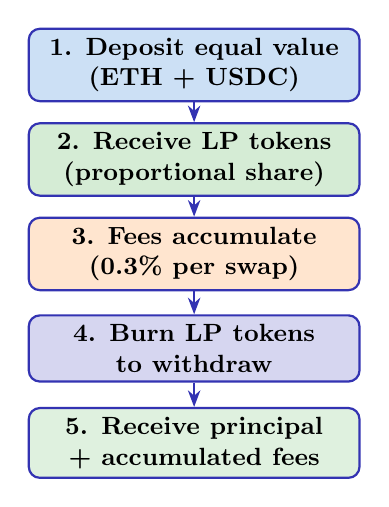
\begin{tikzpicture}[
        stepbox/.style={rectangle, rounded corners=4pt, draw=mlpurple, thick,
                        minimum width=4.2cm, minimum height=0.75cm, align=center,
                        font=\small\bfseries},
        arr/.style={-{Stealth[length=6pt]}, thick, mlpurple}
      ]
        \node[stepbox, fill=mlblue!20]    (s1) at (0, 3.6) {1. Deposit equal value\\(ETH + USDC)};
        \node[stepbox, fill=mlgreen!20]   (s2) at (0, 2.4) {2. Receive LP tokens\\(proportional share)};
        \node[stepbox, fill=mlorange!20]  (s3) at (0, 1.2) {3. Fees accumulate\\(0.3\% per swap)};
        \node[stepbox, fill=mlpurple!20]  (s4) at (0, 0.0) {4. Burn LP tokens\\to withdraw};
        \node[stepbox, fill=mlgreen!15]   (s5) at (0,-1.2) {5. Receive principal\\+ accumulated fees};

        \draw[arr] (s1.south) -- (s2.north);
        \draw[arr] (s2.south) -- (s3.north);
        \draw[arr] (s3.south) -- (s4.north);
        \draw[arr] (s4.south) -- (s5.north);
      \end{tikzpicture}
    \end{column}
    \begin{column}{0.46\textwidth}
      \begin{block}{LP Share Mathematics}
        When depositing $(\Delta x, \Delta y)$ into a pool with reserves $(x, y)$ and total LP supply $S$:
        \[
          \text{LP tokens received} = S \cdot \frac{\Delta x}{x} = S \cdot \frac{\Delta y}{y}
        \]
        \textit{(Both ratios must be equal to maintain the price.)}
      \end{block}
      \vspace{3mm}
      \begin{block}{Fee Revenue}
        \[
          r_{\text{LP}} = \frac{\text{LP share} \times \text{fee} \times \text{volume}}{\text{Total liquidity}}
        \]
        Uniswap V2: fee $= 0.3\%$ of each swap. Fees increase $k$, benefiting all LPs proportionally.
      \end{block}
      \vspace{3mm}
      \begin{alertblock}{Risk}
        LPs face \textbf{impermanent loss} when prices diverge from the deposit ratio (see Frame 24).
      \end{alertblock}
    \end{column}
  \end{columns}
  \bottomnote{LP tokens represent a claim on a fraction of the pool; their value grows with fee income but may fall from impermanent loss}
\end{frame}

% Frame 22: Uniswap V2 vs V3
\begin{frame}[fragile]{Uniswap V2 vs.\ V3: Concentrated Liquidity}
  \begin{columns}[T]
    \begin{column}{0.46\textwidth}
      \vspace{2mm}
      \textbf{V2: Full-Range Liquidity}
      \vspace{2mm}

      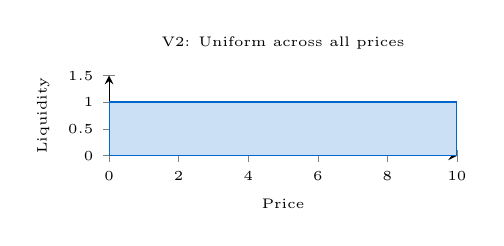
\begin{tikzpicture}
        \begin{axis}[
          width=6.0cm, height=2.6cm,
          xmin=0, xmax=10,
          ymin=0, ymax=1.5,
          xlabel={Price},
          ylabel={Liquidity},
          xlabel style={font=\tiny},
          ylabel style={font=\tiny},
          xticklabel style={font=\tiny},
          yticklabel style={font=\tiny},
          axis lines=left,
          title={\tiny V2: Uniform across all prices},
          title style={font=\tiny},
          ytick={0,0.5,1.0,1.5},
          xtick={0,2,4,6,8,10},
        ]
          \addplot[thick, mlblue, fill=mlblue!20]
            coordinates {(0,1.0) (10,1.0)} \closedcycle;
        \end{axis}
      \end{tikzpicture}

      \vspace{1mm}
      \textbf{V3: Concentrated Liquidity}
      \vspace{2mm}

      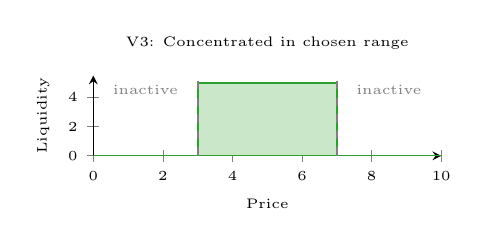
\begin{tikzpicture}
        \begin{axis}[
          width=6.0cm, height=2.6cm,
          xmin=0, xmax=10,
          ymin=0, ymax=5.5,
          xlabel={Price},
          ylabel={Liquidity},
          xlabel style={font=\tiny},
          ylabel style={font=\tiny},
          xticklabel style={font=\tiny},
          yticklabel style={font=\tiny},
          axis lines=left,
          title={\tiny V3: Concentrated in chosen range},
          title style={font=\tiny},
          ytick={0,2,4},
          xtick={0,2,4,6,8,10},
        ]
          \addplot[thick, mlgreen, fill=mlgreen!25]
            coordinates {(0,0) (3,0) (3,5.0) (7,5.0) (7,0) (10,0)} \closedcycle;
          \addplot[dashed, mlgray, thick] coordinates {(3,0) (3,5.5)};
          \addplot[dashed, mlgray, thick] coordinates {(7,0) (7,5.5)};
          \node[font=\tiny, mlgray] at (axis cs:1.5, 4.5) {inactive};
          \node[font=\tiny, mlgray] at (axis cs:8.5, 4.5) {inactive};
        \end{axis}
      \end{tikzpicture}
    \end{column}
    \begin{column}{0.50\textwidth}
\begin{lstlisting}[language=Solidity, caption={}]
// SPDX-License-Identifier: MIT
pragma solidity ^0.8.0;

// Uniswap V3: Concentrated Liquidity
struct Position {
    uint128 liquidity;
    int24 tickLower;  // Price range start
    int24 tickUpper;  // Price range end
}

// V2: liquidity spread 0 to infinity
// V3: liquidity in [tickLower, tickUpper]
// Result: up to 4000x capital efficiency
\end{lstlisting}
      \vspace{3mm}
      \begin{block}{V2 vs.\ V3 Key Differences}
        \begin{tabular}{lll}
          \toprule
          & \textbf{V2} & \textbf{V3} \\
          \midrule
          Range     & $[0, \infty)$ & $[a, b]$ chosen \\
          Efficiency& 1$\times$     & up to 4000$\times$ \\
          Fee tiers & 0.3\%         & 0.05/0.3/1\%  \\
          IL risk   & Lower         & Higher (in range) \\
          \bottomrule
        \end{tabular}
      \end{block}
    \end{column}
  \end{columns}
  \bottomnote{V3 concentrated liquidity dramatically improves capital efficiency but requires active management of price ranges}
\end{frame}

% Frame 23: Other AMM Models
\begin{frame}{Other AMM Models}
  \begin{columns}[T]
    \begin{column}{0.54\textwidth}
      \centering
      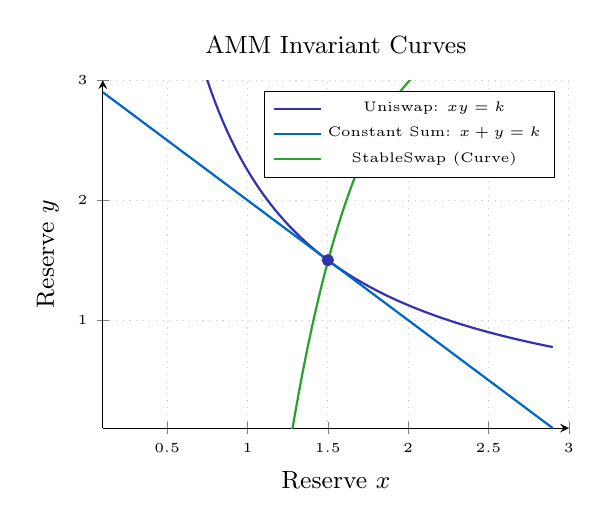
\begin{tikzpicture}
        \begin{axis}[
          width=7.5cm, height=6.0cm,
          xmin=0.1, xmax=3.0,
          ymin=0.1, ymax=3.0,
          xlabel={Reserve $x$},
          ylabel={Reserve $y$},
          xlabel style={font=\small},
          ylabel style={font=\small},
          xticklabel style={font=\tiny},
          yticklabel style={font=\tiny},
          axis lines=left,
          grid=major,
          grid style={dotted, mlgray!40},
          title={\small AMM Invariant Curves},
          title style={font=\small},
          legend pos=north east,
          legend style={font=\tiny},
        ]
          % Constant Product: xy = 1.5^2 = 2.25
          \addplot[thick, mlpurple, domain=0.12:2.9, samples=120] {2.25/x};
          \addlegendentry{Uniswap: $xy=k$}
          % Constant Sum: x + y = 3 (line from (0.1,2.9) to (2.9,0.1))
          \addplot[thick, mlblue, domain=0.1:2.9, samples=2] {3 - x};
          \addlegendentry{Constant Sum: $x+y=k$}
          % StableSwap hybrid (Curve-like approximation: steeper near midpoint)
          % Approximation: solve A*(x+y) + xy = A*2*1.5 + 1.5^2 around x=y=1.5
          % Use parametric approximation along the curve
          \addplot[thick, mlgreen, domain=0.4:2.6, samples=80]
            {(2.25 + 6*(x-1.5)*(1.5) - (x-1.5)^2*3) / (x + 0.01)};
          \addlegendentry{StableSwap (Curve)}
          % Mark midpoints
          \addplot[only marks, mark=*, mark options={fill=mlpurple, draw=mlpurple}, mark size=2pt]
            coordinates {(1.5, 1.5)};
        \end{axis}
      \end{tikzpicture}
    \end{column}
    \begin{column}{0.42\textwidth}
      \begin{block}{Constant Product (Uniswap)}
        $x \cdot y = k$ --- Hyperbola. Works for any token pair. Price adjusts continuously.
      \end{block}
      \vspace{3mm}
      \begin{block}{Constant Sum}
        $x + y = k$ --- Straight line. Zero price impact but \textbf{pool drainable}: arbitrageurs
        empty one side entirely.
      \end{block}
      \vspace{3mm}
      \begin{block}{StableSwap (Curve)}
        Hybrid between constant sum and constant product:
        \[
          A(x+y) + xy = A \cdot D + \left(\frac{D}{2}\right)^2
        \]
        Near-zero slippage near the peg; reverts to constant product at extremes. Optimal for
        stablecoin swaps (USDC/USDT/DAI).
      \end{block}
    \end{column}
  \end{columns}
  \bottomnote{AMM design is a trilemma: capital efficiency, price stability near peg, and resistance to pool depletion}
\end{frame}

% Frame 24: Impermanent Loss Math
\begin{frame}{Impermanent Loss: Derivation and Magnitude}
  \begin{columns}[T]
    \begin{column}{0.48\textwidth}
      \begin{block}{IL Derivation}
        Let $r = P_1 / P_0$ be the price ratio (current vs.\ entry).\\[4pt]
        Value of LP position after price change (per unit of initial capital):
        \[
          V_{\text{LP}} = 2 \sqrt{r}
        \]
        Value if simply held (50/50 split):
        \[
          V_{\text{HODL}} = 1 + r
        \]
        Impermanent Loss:
        \[
          \boxed{IL(r) = \frac{2\sqrt{r}}{1+r} - 1}
        \]
      \end{block}
      \vspace{3mm}
      \begin{block}{Key Values}
        \begin{tabular}{lll}
          \toprule
          Price ratio $r$ & IL & Example \\
          \midrule
          1.0 & 0.00\%    & No change \\
          1.25 & $-$0.57\% & ETH $+$25\% \\
          2.0  & $-$5.72\% & ETH $\times$2 \\
          4.0  & $-$20.0\% & ETH $\times$4 \\
          0.5  & $-$5.72\% & ETH $-$50\% \\
          \bottomrule
        \end{tabular}
      \end{block}
    \end{column}
    \begin{column}{0.48\textwidth}
      \centering
      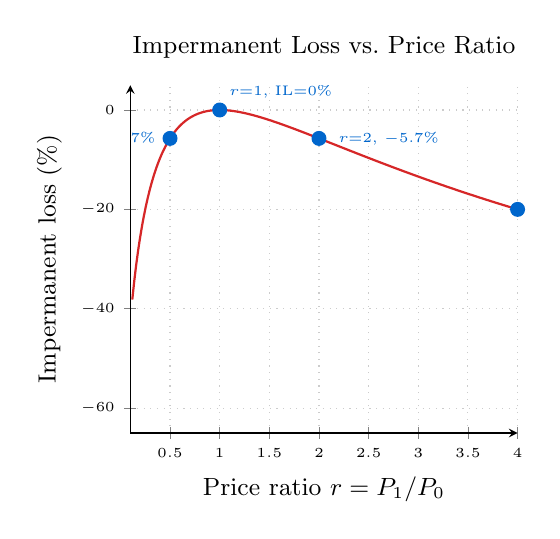
\begin{tikzpicture}
        \begin{axis}[
          width=6.5cm, height=6.0cm,
          xmin=0.1, xmax=4.0,
          ymin=-65, ymax=5,
          xlabel={Price ratio $r = P_1/P_0$},
          ylabel={Impermanent loss (\%)},
          xlabel style={font=\small},
          ylabel style={font=\small},
          xticklabel style={font=\tiny},
          yticklabel style={font=\tiny},
          axis lines=left,
          grid=major,
          grid style={dotted, mlgray!40},
          title={\small Impermanent Loss vs.\ Price Ratio},
          title style={font=\small},
          xtick={0.5,1,1.5,2,2.5,3,3.5,4},
        ]
          \addplot[thick, mlred, domain=0.12:4.0, samples=200]
            {(2*sqrt(x)/(1+x) - 1)*100};
          % Key annotation points
          \addplot[only marks, mark=*, mark options={fill=mlblue, draw=mlblue}, mark size=2.5pt]
            coordinates {(1.0, 0.0) (2.0, -5.72) (4.0, -20.0) (0.5, -5.72)};
          \node[font=\tiny, mlblue, anchor=south west] at (axis cs:1.0,  0.5) {$r$=1, IL=0\%};
          \node[font=\tiny, mlblue, anchor=west]       at (axis cs:2.1, -5.72) {$r$=2, $-$5.7\%};
          \node[font=\tiny, mlblue, anchor=west]       at (axis cs:4.05,-20.0) {$r$=4, $-$20\%};
          \node[font=\tiny, mlblue, anchor=east]       at (axis cs:0.45,-5.72) {$r$=0.5, $-$5.7\%};
        \end{axis}
      \end{tikzpicture}
    \end{column}
  \end{columns}
  \bottomnote{IL is ``impermanent'' only if prices revert; it becomes permanent upon withdrawal and must be offset by fee income}
\end{frame}

% Frame 25: DEX Aggregators
\begin{frame}{DEX Aggregators: Optimal Order Routing}
  \centering
  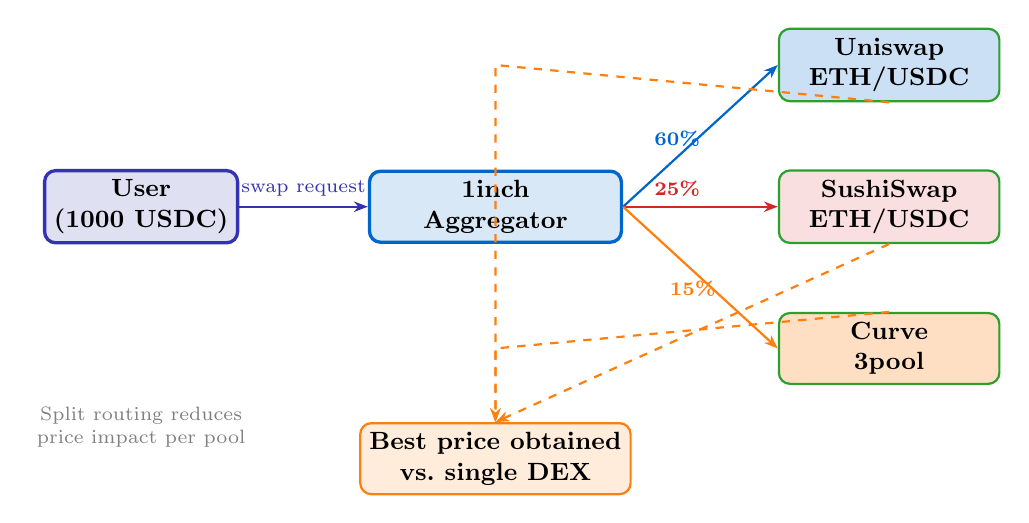
\begin{tikzpicture}[
    userbox/.style={rectangle, rounded corners=4pt, draw=mlpurple, very thick,
                    minimum width=2.4cm, minimum height=0.9cm, align=center,
                    font=\small\bfseries, fill=mlpurple!15},
    aggbox/.style={rectangle, rounded corners=4pt, draw=mlblue, very thick,
                   minimum width=3.2cm, minimum height=0.9cm, align=center,
                   font=\small\bfseries, fill=mlblue!15},
    dexbox/.style={rectangle, rounded corners=4pt, draw=mlgreen, thick,
                   minimum width=2.8cm, minimum height=0.8cm, align=center,
                   font=\small\bfseries},
    resultbox/.style={rectangle, rounded corners=4pt, draw=mlorange, thick,
                      minimum width=3.2cm, minimum height=0.9cm, align=center,
                      font=\small\bfseries, fill=mlorange!15},
    pctlbl/.style={rectangle, fill=mlgray!15, rounded corners=2pt,
                   minimum width=1.2cm, minimum height=0.45cm, align=center,
                   font=\scriptsize\bfseries},
    arr/.style={-{Stealth[length=5pt]}, thick}
  ]
    % User
    \node[userbox]   (user) at (0, 0) {User\\(1000 USDC)};
    % Aggregator
    \node[aggbox]    (agg)  at (4.5, 0) {1inch\\Aggregator};
    \draw[arr, mlpurple] (user.east) -- (agg.west) node[midway, above, font=\scriptsize] {swap request};

    % DEX branches
    \node[dexbox, fill=mlblue!20]   (uni) at (9.5, 1.8) {Uniswap\\ETH/USDC};
    \node[dexbox, fill=mlred!15]    (sus) at (9.5, 0.0) {SushiSwap\\ETH/USDC};
    \node[dexbox, fill=mlorange!25] (crv) at (9.5,-1.8) {Curve\\3pool};

    \draw[arr, mlblue]   (agg.east) -- (uni.west) node[pos=0.35, above, font=\scriptsize\bfseries, mlblue] {60\%};
    \draw[arr, mlred]    (agg.east) -- (sus.west) node[pos=0.35, above, font=\scriptsize\bfseries, mlred] {25\%};
    \draw[arr, mlorange] (agg.east) -- (crv.west) node[pos=0.45, below, font=\scriptsize\bfseries, mlorange] {15\%};

    % Result
    \node[resultbox] (res) at (4.5,-3.2) {Best price obtained\\vs.\ single DEX};
    \draw[arr, mlorange, dashed] (uni.south)  -- (4.5,1.8)  -- (res.north);
    \draw[arr, mlorange, dashed] (sus.south)  -- (res.north);
    \draw[arr, mlorange, dashed] (crv.north)  -- (4.5,-1.8) -- (res.north);

    % Benefit label
    \node[font=\scriptsize, mlgray, align=center] at (0,-2.8)
      {Split routing reduces\\price impact per pool};
  \end{tikzpicture}
  \bottomnote{Aggregators like 1inch, Paraswap, and CoW Protocol split orders across multiple pools to minimise total price impact}
\end{frame}

% Frame 26: Section 2 Summary
\begin{frame}{Section 2 Summary: DEXs and AMMs}
  \begin{columns}[T]
    \begin{column}{0.48\textwidth}
      \begin{block}{Key Takeaways}
        \begin{enumerate}\setlength\itemsep{4pt}
          \item \textbf{AMMs replace order books} with pooled reserves and a mathematical invariant,
                enabling instant, permissionless trades against the pool
          \item \textbf{Constant product} $x \cdot y = k$ sets price via reserve ratio; every trade
                moves along the hyperbola, causing price impact
          \item \textbf{Price impact scales super-linearly} with trade size relative to pool depth;
                aggregators mitigate this by splitting routes
          \item \textbf{Liquidity providers} earn fees proportional to their share but face
                impermanent loss when prices diverge from entry
          \item \textbf{V3 concentrated liquidity} multiplies capital efficiency up to 4000$\times$
                but requires active range management
        \end{enumerate}
      \end{block}
    \end{column}
    \begin{column}{0.48\textwidth}
      \begin{block}{Formulas to Remember}
        \[
          x \cdot y = k \quad \text{(constant product)}
        \]
        \[
          \Delta y = y_0 - \frac{k}{x_0 + \Delta x} \quad \text{(amount out)}
        \]
        \[
          IL(r) = \frac{2\sqrt{r}}{1+r} - 1 \quad \text{(impermanent loss)}
        \]
        \[
          \text{LP share} = S \cdot \frac{\Delta x}{x} \quad \text{(LP tokens)}
        \]
      \end{block}
      \vspace{3mm}
      \begin{alertblock}{Coming Up: Section 3}
        Lending and Borrowing --- interest rate curves, collateral mechanics, and liquidation
        mathematics on Aave and Compound.
      \end{alertblock}
    \end{column}
  \end{columns}
  \bottomnote{Section 2 complete | Next: Section 3 --- Lending and Borrowing | Frames 27 onward}
\end{frame}

%% ============================================================
%% SECTION 3: Lending and Borrowing
%% ============================================================

\section{Lending \& Borrowing}

% Frame 27: Section Divider
\begin{frame}
  \begin{beamercolorbox}[sep=12pt,center,rounded=true,shadow=true]{palette quaternary}
    {\Large\bfseries Section 3: Lending and Borrowing}\\{}\vspace{6pt}
    {\normalsize Collateralisation, interest rate models, liquidation mechanics, and protocol architecture}
  \end{beamercolorbox}
  \vspace{8mm}
  \begin{columns}[T]
    \begin{column}{0.48\textwidth}
      \begin{block}{What you will learn}
        \begin{itemize}\setlength\itemsep{2pt}
          \item How DeFi lending pools work end-to-end
          \item Collateralisation ratios and loan-to-value limits
          \item Kinked interest rate models and utilisation-driven pricing
          \item Health factor computation and liquidation triggers
          \item Aave vs.\ Compound architecture differences
        \end{itemize}
      \end{block}
    \end{column}
    \begin{column}{0.48\textwidth}
      \begin{block}{Frames in this section}
        \begin{itemize}\setlength\itemsep{2pt}
          \item Frame 28 -- How DeFi Lending Works
          \item Frame 29 -- Collateralisation Ratios
          \item Frames 30--31 -- Interest Rate Models
          \item Frames 32--33 -- Liquidation Mechanics, Health Factor
          \item Frames 34--38 -- Protocol Architecture, Stablecoins, Summary
        \end{itemize}
      \end{block}
    \end{column}
  \end{columns}
  \bottomnote{Section 3 | Frames 27--38 | Lending and Borrowing}
\end{frame}

% Frame 28: How DeFi Lending Works
\begin{frame}{How DeFi Lending Works}
  \centering
  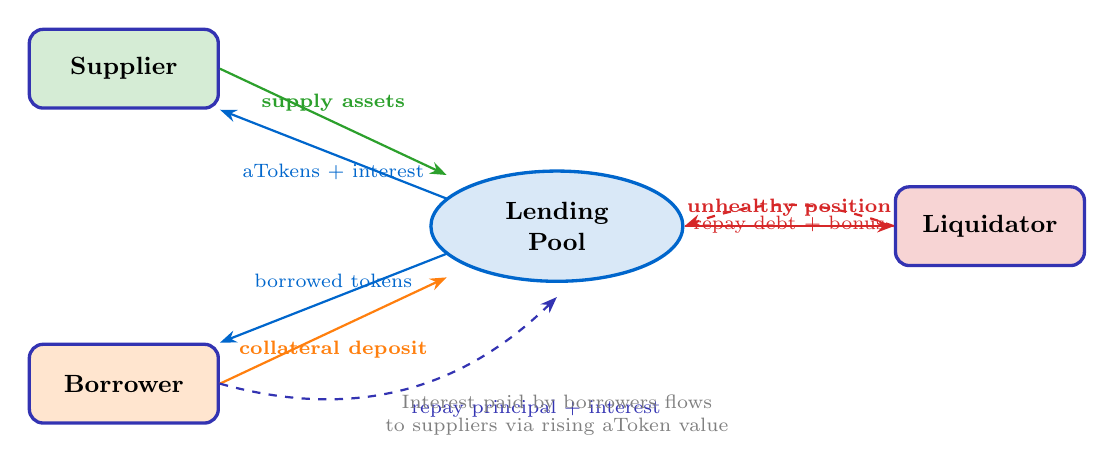
\begin{tikzpicture}[
    actorbox/.style={rectangle, rounded corners=5pt, draw=mlpurple, very thick,
                     minimum width=2.4cm, minimum height=1.0cm, align=center,
                     font=\small\bfseries},
    poolbox/.style={ellipse, draw=mlblue, very thick, fill=mlblue!15,
                    minimum width=3.2cm, minimum height=1.4cm, align=center,
                    font=\small\bfseries},
    arr/.style={-{Stealth[length=6pt]}, thick}
  ]
    % Central pool
    \node[poolbox] (pool) at (0, 0) {Lending\\Pool};

    % Supplier
    \node[actorbox, fill=mlgreen!20]  (sup) at (-5.5, 2.0) {Supplier};
    % Borrower
    \node[actorbox, fill=mlorange!20] (bor) at (-5.5,-2.0) {Borrower};
    % Liquidator
    \node[actorbox, fill=mlred!20]    (liq) at ( 5.5, 0.0) {Liquidator};

    % Supplier -> Pool: supply assets
    \draw[arr, mlgreen]  (sup.east)  -- node[above, font=\scriptsize\bfseries, mlgreen]  {supply assets} (-1.4, 0.65);
    % Pool -> Supplier: aTokens + interest
    \draw[arr, mlblue]   (-1.4, 0.35) -- node[below, font=\scriptsize, mlblue] {aTokens + interest} (sup.south east);

    % Borrower -> Pool: collateral
    \draw[arr, mlorange] (bor.east)  -- node[below, font=\scriptsize\bfseries, mlorange] {collateral deposit} (-1.4,-0.65);
    % Pool -> Borrower: borrowed tokens
    \draw[arr, mlblue]   (-1.4,-0.35) -- node[above, font=\scriptsize, mlblue] {borrowed tokens} (bor.north east);
    % Borrower -> Pool: repay + interest
    \draw[arr, mlpurple, dashed] (bor.east) to[bend right=30]
      node[below right, font=\scriptsize, mlpurple] {repay principal + interest} (0,-0.9);

    % Liquidator
    \draw[arr, mlred]    (pool.east) -- node[above, font=\scriptsize\bfseries, mlred]  {unhealthy position} (liq.west);
    \draw[arr, mlred, dashed] (liq.west) to[bend right=20]
      node[below, font=\scriptsize, mlred] {repay debt + bonus} (pool.east);

    % Interest flow note
    \node[font=\scriptsize, mlgray, align=center] at (0,-2.4)
      {Interest paid by borrowers flows\\to suppliers via rising aToken value};
  \end{tikzpicture}
  \bottomnote{Lending pools intermediary-free: suppliers earn yield while borrowers access liquidity against locked collateral}
\end{frame}

% Frame 29: Collateralisation Ratios
\begin{frame}{Collateralisation Ratios}
  \begin{columns}[T]
    \begin{column}{0.48\textwidth}
      \centering
      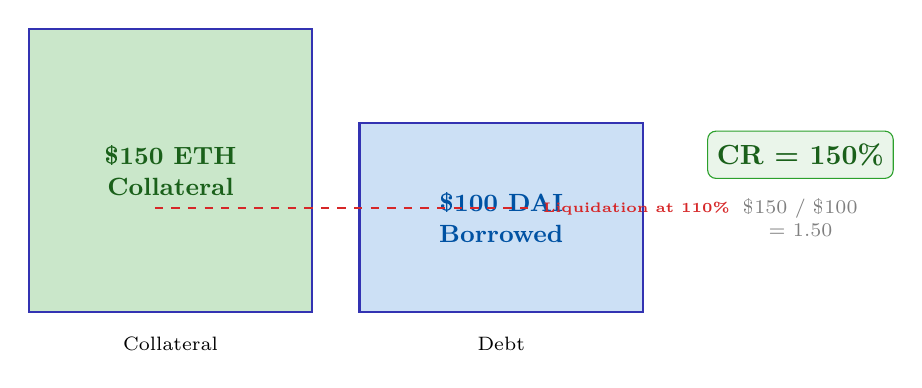
\begin{tikzpicture}[
        barbox/.style={rectangle, draw=mlpurple, thick, minimum width=3.6cm, align=center,
                       font=\small\bfseries},
        lbl/.style={font=\scriptsize, align=center}
      ]
        % Collateral bar: $150 ETH
        \node[barbox, minimum height=3.6cm, fill=mlgreen!25]  (col) at (0, 1.8) {};
        \node[font=\small\bfseries, mlgreen!60!black, align=center] at (0, 1.8) {\$150 ETH\\Collateral};

        % Borrowed bar: $100 DAI
        \node[barbox, minimum height=2.4cm, fill=mlblue!20]   (bor) at (4.2, 1.2) {};
        \node[font=\small\bfseries, mlblue!80!black, align=center] at (4.2, 1.2) {\$100 DAI\\Borrowed};

        % Danger zone marker
        \draw[thick, mlred, dashed] (-0.2, 1.32) -- (4.6, 1.32)
          node[right, font=\tiny\bfseries, mlred] {Liquidation at 110\%};

        % Ratio annotation
        \node[font=\normalsize\bfseries, mlgreen!60!black,
              draw=mlgreen, rounded corners=3pt, fill=mlgreen!10,
              minimum width=2.0cm, minimum height=0.6cm, align=center]
          at (8.0, 2.0) {CR = 150\%};
        \node[font=\scriptsize, mlgray, align=center] at (8.0, 1.2)
          {\$150 / \$100\\= 1.50};

        % x-axis labels
        \node[lbl] at (0,  -0.4) {Collateral};
        \node[lbl] at (4.2,-0.4) {Debt};
      \end{tikzpicture}

      \vspace{4mm}
      \footnotesize
      \[
        CR = \frac{V_{\text{collateral}}}{V_{\text{debt}}} \qquad \text{LTV} = \frac{V_{\text{debt}}}{V_{\text{collateral}}}
      \]
    \end{column}
    \begin{column}{0.48\textwidth}
      \begin{block}{Aave V3 Risk Parameters (illustrative)}
        \begin{center}
        \footnotesize
        \begin{tabular}{lccc}
          \toprule
          \textbf{Asset} & \textbf{Max LTV} & \textbf{Liq. Threshold} & \textbf{Liq. Penalty} \\
          \midrule
          ETH   & 80.0\% & 82.5\% & 5.0\%   \\
          WBTC  & 70.0\% & 75.0\% & 6.25\%  \\
          USDC  & 77.0\% & 80.0\% & 4.5\%   \\
          DAI   & 77.0\% & 80.0\% & 4.5\%   \\
          LINK  & 65.0\% & 70.0\% & 7.5\%   \\
          \bottomrule
        \end{tabular}
        \end{center}
      \end{block}
      \vspace{3mm}
      \begin{alertblock}{Key Insight}
        The \textbf{liquidation threshold} is always above the \textbf{max LTV}, giving a safety buffer.
        A borrower depositing \$100 of ETH can borrow at most \$80 (80\% LTV) but faces liquidation
        only if the position degrades past the 82.5\% threshold.
      \end{alertblock}
    \end{column}
  \end{columns}
  \bottomnote{Over-collateralisation is the primary solvency mechanism in DeFi lending; there is no recourse for undercollateralised default}
\end{frame}

% Frame 30: Interest Rate Models
\begin{frame}{Interest Rate Models}
  \begin{columns}[T]
    \begin{column}{0.54\textwidth}
      \centering
      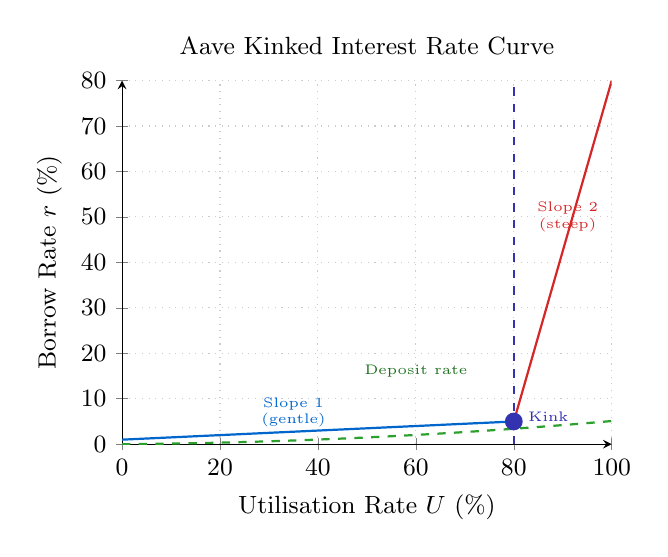
\begin{tikzpicture}
        \begin{axis}[
          width=7.8cm, height=6.2cm,
          xmin=0, xmax=100,
          ymin=0, ymax=80,
          xlabel={Utilisation Rate $U$ (\%)},
          ylabel={Borrow Rate $r$ (\%)},
          xlabel style={font=\small},
          ylabel style={font=\small},
          xticklabel style={font=\small},
          yticklabel style={font=\small},
          axis lines=left,
          grid=major,
          grid style={dotted, mlgray!40},
          title={\small Aave Kinked Interest Rate Curve},
          title style={font=\small},
          xtick={0,20,40,60,80,100},
          ytick={0,10,20,30,40,50,60,70,80},
        ]
          % Below optimal (0 to 80%): baseRate=1, slope1=4 => r = 1 + (U/80)*4
          \addplot[thick, mlblue, domain=0:80, samples=81]
            {1 + (x/80)*4};
          % Above optimal (80 to 100%): r = 5 + ((U-80)/20)*75
          \addplot[thick, mlred, domain=80:100, samples=21]
            {5 + ((x-80)/20)*75};
          % Optimal utilisation marker
          \draw[dashed, thick, mlpurple] (axis cs:80,0) -- (axis cs:80,80)
            node[above, font=\tiny\bfseries, mlpurple] {$U^*=80\%$};
          % Kink point marker
          \addplot[only marks, mark=*, mark options={fill=mlpurple, draw=mlpurple}, mark size=3pt]
            coordinates {(80, 5)};
          \node[font=\tiny, mlpurple, anchor=west] at (axis cs:81, 6) {Kink};
          % Labels
          \node[font=\tiny, mlblue,  align=center] at (axis cs:35,  7) {Slope 1\\(gentle)};
          \node[font=\tiny, mlred, align=center]   at (axis cs:91, 50) {Slope 2\\(steep)};
          % Deposit rate approximation
          \addplot[thick, mlgreen, dashed, domain=0:100, samples=101]
            {0.85 * (1 + (x/80)*4) * (x/100)};
          \node[font=\tiny, mlgreen!70!black] at (axis cs:60, 16) {Deposit rate};
        \end{axis}
      \end{tikzpicture}
    \end{column}
    \begin{column}{0.42\textwidth}
      \begin{block}{Kinked Rate Rationale}
        The two-slope model achieves three goals simultaneously:
        \begin{enumerate}\setlength\itemsep{3pt}
          \item \textbf{Low rates at low utilisation} attract borrowers and grow the market
          \item \textbf{Moderate rates near optimal} balance supply and demand efficiently
          \item \textbf{Steep rates above optimal} act as an automatic brake, incentivising
                repayment and new deposits before liquidity is exhausted
        \end{enumerate}
      \end{block}
      \vspace{3mm}
      \begin{block}{Rate Parameters (Aave style)}
        \begin{tabular}{ll}
          \toprule
          Parameter & Value \\
          \midrule
          Base rate      & 1\%  \\
          Optimal util.\ $U^*$ & 80\% \\
          Slope 1 (below $U^*$)    & 4\%  \\
          Slope 2 (above $U^*$)    & 75\% \\
          \bottomrule
        \end{tabular}
      \end{block}
    \end{column}
  \end{columns}
  \bottomnote{The kinked rate curve is the dominant interest rate design in DeFi lending; it self-corrects liquidity without manual intervention}
\end{frame}

% Frame 31: Interest Rate Formula
\begin{frame}{Interest Rate Formula: Mathematics}
  \begin{columns}[T]
    \begin{column}{0.52\textwidth}
      \begin{block}{Piecewise Rate Function}
        Let $U$ = utilisation rate, $U^*$ = optimal utilisation.
        \[
          r_{\text{borrow}}(U) =
          \begin{cases}
            r_{\text{base}} + \dfrac{U}{U^*} \cdot s_1
              & \text{if } U \leq U^* \\[8pt]
            r_{\text{base}} + s_1 + \dfrac{U - U^*}{1 - U^*} \cdot s_2
              & \text{if } U > U^*
          \end{cases}
        \]
        where $s_1$ = slope~1, $s_2$ = slope~2.
      \end{block}
      \vspace{3mm}
      \begin{block}{Deposit Rate}
        \[
          r_{\text{deposit}} = r_{\text{borrow}} \cdot U \cdot (1 - \text{reserveFactor})
        \]
        The reserve factor (e.g., 10\%) accrues to the protocol treasury.
      \end{block}
      \vspace{3mm}
      \begin{block}{Worked Example ($U = 60\%$)}
        $r_{\text{borrow}} = 1\% + \tfrac{0.60}{0.80} \times 4\% = 1\% + 3\% = \mathbf{4\%}$\\[4pt]
        $r_{\text{deposit}} = 4\% \times 0.60 \times 0.90 = \mathbf{2.16\%}$
      \end{block}
    \end{column}
    \begin{column}{0.44\textwidth}
      \centering
      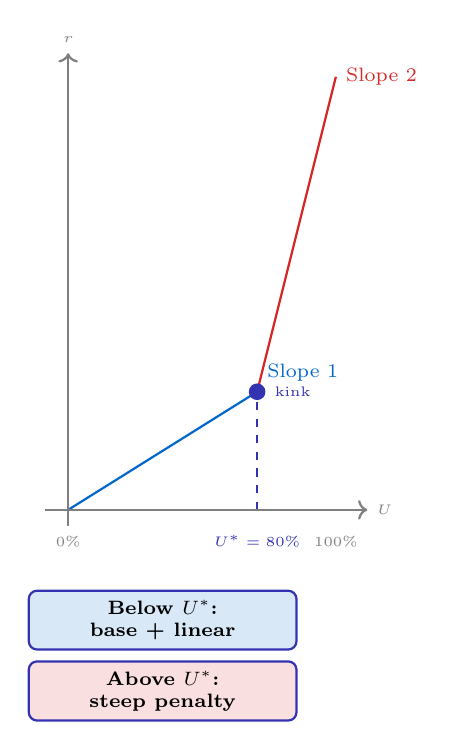
\begin{tikzpicture}[
        lblbox/.style={rectangle, rounded corners=3pt, draw=mlpurple, thick,
                       minimum width=3.4cm, minimum height=0.65cm, align=center,
                       font=\scriptsize\bfseries},
        arr/.style={-{Stealth[length=5pt]}, thick, mlpurple}
      ]
        % Kink visualisation
        \draw[thick, mlblue] (0,0) -- (2.4,1.5)
          node[above right, font=\scriptsize, mlblue] {Slope 1};
        \draw[thick, mlred]  (2.4,1.5) -- (3.4,5.5)
          node[right, font=\scriptsize, mlred] {Slope 2};
        \draw[dashed, mlpurple, thick] (2.4,0) -- (2.4,1.5);
        \node[font=\tiny\bfseries, mlpurple] at (2.4,-0.4) {$U^*=80\%$};
        \node[font=\tiny, mlgray] at (0,-0.4) {0\%};
        \node[font=\tiny, mlgray] at (3.4,-0.4) {100\%};
        \draw[thick, mlgray, ->] (-0.3,0) -- (3.8,0) node[right, font=\tiny] {$U$};
        \draw[thick, mlgray, ->] (0,-0.2) -- (0,5.8) node[above, font=\tiny] {$r$};
        % Kink dot
        \fill[mlpurple] (2.4,1.5) circle (3pt);
        \node[font=\tiny, mlpurple, anchor=west] at (2.5,1.5) {kink};
        % Annotations
        \node[lblbox, fill=mlblue!15, align=center] at (1.2,-1.4)
          {Below $U^*$:\\base + linear};
        \node[lblbox, fill=mlred!15, align=center]  at (1.2,-2.3)
          {Above $U^*$:\\steep penalty};
      \end{tikzpicture}
    \end{column}
  \end{columns}
  \bottomnote{Interest accrues every block in Ethereum; the continuous compounding effect means rates quoted as APR differ from effective APY}
\end{frame}

% Frame 32: Liquidation Mechanics
\begin{frame}{Liquidation Mechanics}
  \centering
  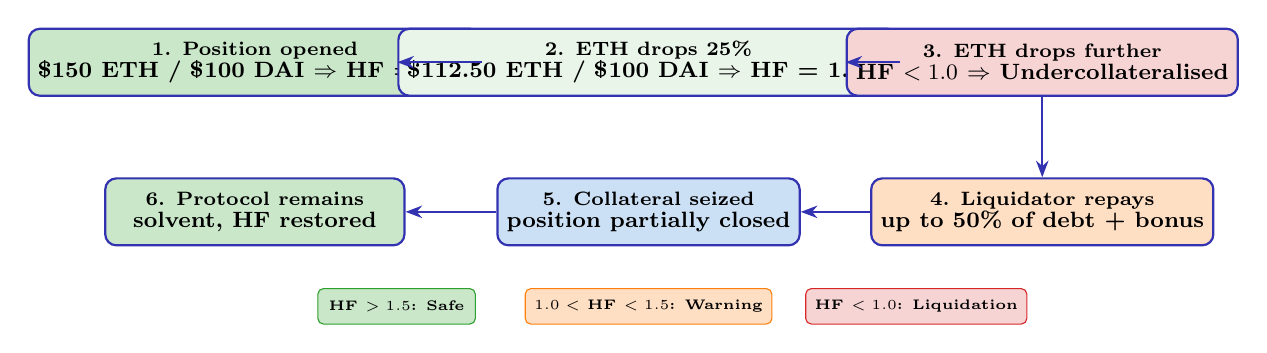
\begin{tikzpicture}[
    stepbox/.style={rectangle, rounded corners=4pt, draw=mlpurple, thick,
                    minimum width=3.8cm, minimum height=0.85cm, align=center,
                    font=\scriptsize\bfseries},
    arr/.style={-{Stealth[length=6pt]}, thick, mlpurple}
  ]
    % Step 1: healthy position
    \node[stepbox, fill=mlgreen!25]  (s1) at (0,    0) {1. Position opened\\{\footnotesize\$150 ETH / \$100 DAI $\Rightarrow$ HF = 1.50}};
    % Step 2: ETH drops 25%
    \node[stepbox, fill=mlgreen!10]  (s2) at (5.0,  0) {2. ETH drops 25\%\\{\footnotesize\$112.50 ETH / \$100 DAI $\Rightarrow$ HF = 1.125}};
    % Step 3: HF < 1
    \node[stepbox, fill=mlred!20]    (s3) at (10.0, 0) {3. ETH drops further\\{\footnotesize HF $< 1.0$ $\Rightarrow$ Undercollateralised}};
    % Step 4: liquidator acts
    \node[stepbox, fill=mlorange!25] (s4) at (10.0,-1.9) {4. Liquidator repays\\{\footnotesize up to 50\% of debt + bonus}};
    % Step 5: position reduced
    \node[stepbox, fill=mlblue!20]   (s5) at (5.0, -1.9) {5. Collateral seized\\{\footnotesize position partially closed}};
    % Step 6: protocol solvent
    \node[stepbox, fill=mlgreen!25]  (s6) at (0,   -1.9) {6. Protocol remains\\{\footnotesize solvent, HF restored}};

    \draw[arr] (s1.east) -- (s2.west);
    \draw[arr] (s2.east) -- (s3.west);
    \draw[arr] (s3.south) -- (s4.north);
    \draw[arr] (s4.west) -- (s5.east);
    \draw[arr] (s5.west) -- (s6.east);

    % Color zone legend
    \node[rectangle, fill=mlgreen!25,  draw=mlgreen,  rounded corners=2pt,
          minimum width=2.0cm, minimum height=0.45cm, align=center, font=\tiny\bfseries]
      at (1.8, -3.1) {HF $> 1.5$: Safe};
    \node[rectangle, fill=mlorange!25, draw=mlorange, rounded corners=2pt,
          minimum width=2.4cm, minimum height=0.45cm, align=center, font=\tiny\bfseries]
      at (5.0, -3.1) {$1.0 < $ HF $ < 1.5$: Warning};
    \node[rectangle, fill=mlred!20,    draw=mlred,    rounded corners=2pt,
          minimum width=2.0cm, minimum height=0.45cm, align=center, font=\tiny\bfseries]
      at (8.4, -3.1) {HF $< 1.0$: Liquidation};
  \end{tikzpicture}
  \bottomnote{Liquidations are permissionless: any wallet can repay a borrower's debt and claim collateral at a discount; this incentivises rapid execution}
\end{frame}

% Frame 33: Health Factor Deep Dive
\begin{frame}{Health Factor: Deep Dive}
  \begin{columns}[T]
    \begin{column}{0.50\textwidth}
      \begin{block}{Health Factor Formula}
        \[
          HF = \frac{\displaystyle\sum_{i} V_{c,i} \cdot LT_i}{V_{\text{debt,total}}}
        \]
        where $V_{c,i}$ is the USD value of collateral asset $i$ and $LT_i$ is its liquidation threshold.
        Liquidation is triggered when $HF < 1$.
      \end{block}
      \vspace{3mm}
      \begin{block}{Multi-Asset Example}
        \footnotesize
        \begin{tabular}{lcccc}
          \toprule
          Asset & Value & LT & Weighted \\
          \midrule
          ETH  & \$1{,}000 & 82.5\% & \$825.00 \\
          WBTC & \$500   & 75.0\% & \$375.00 \\
          \midrule
          \multicolumn{3}{l}{Total weighted collateral} & \$1{,}200.00 \\
          \multicolumn{3}{l}{Total debt (DAI)} & \$800.00 \\
          \midrule
          \multicolumn{3}{l}{\textbf{Health Factor}} & \textbf{1.50} \\
          \bottomrule
        \end{tabular}
      \end{block}
    \end{column}
    \begin{column}{0.46\textwidth}
      \centering
      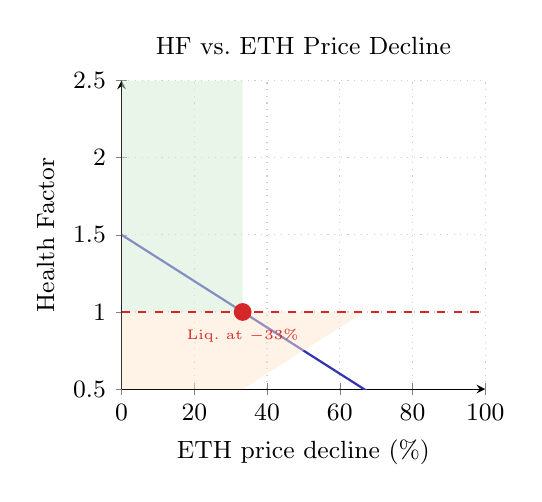
\begin{tikzpicture}
        \begin{axis}[
          width=6.2cm, height=5.5cm,
          xmin=0, xmax=100,
          ymin=0.5, ymax=2.5,
          xlabel={ETH price decline (\%)},
          ylabel={Health Factor},
          xlabel style={font=\small},
          ylabel style={font=\small},
          xticklabel style={font=\small},
          yticklabel style={font=\small},
          axis lines=left,
          grid=major,
          grid style={dotted, mlgray!40},
          title={\small HF vs.\ ETH Price Decline},
          title style={font=\small},
          xtick={0,20,40,60,80,100},
        ]
          % HF = 1.50 * (1 - x/100), starting from HF=1.5 at x=0
          \addplot[thick, mlpurple, domain=0:100, samples=101] {1.50*(1-x/100)};
          % Safe zone fill
          \addplot[fill=mlgreen!20, draw=none, opacity=0.5]
            coordinates {(0,1.5) (0,2.5) (33.3,2.5) (33.3,1.0) (0,1.0)} \closedcycle;
          % Warning zone
          \addplot[fill=mlorange!20, draw=none, opacity=0.5]
            coordinates {(0,1.0) (33.3,1.0) (66.7,1.0) (33.3,0.5) (0,0.5)} \closedcycle;
          % Liquidation line
          \draw[dashed, thick, mlred] (axis cs:0,1.0) -- (axis cs:100,1.0)
            node[right, font=\tiny\bfseries, mlred] {HF=1};
          % Liquidation point
          \addplot[only marks, mark=*, mark options={fill=mlred, draw=mlred}, mark size=3pt]
            coordinates {(33.3, 1.0)};
          \node[font=\tiny, mlred, anchor=north] at (axis cs:33.3, 0.95)
            {Liq.\ at $-$33\%};
        \end{axis}
      \end{tikzpicture}
    \end{column}
  \end{columns}
  \bottomnote{Health factor aggregates multiple collateral assets with asset-specific thresholds; monitoring HF is essential for active borrowers}
\end{frame}

% Frame 34: Aave Protocol Architecture [FRAGILE]
\begin{frame}[fragile]{Aave Protocol Architecture}
  \begin{columns}[T]
    \begin{column}{0.46\textwidth}
      \centering
      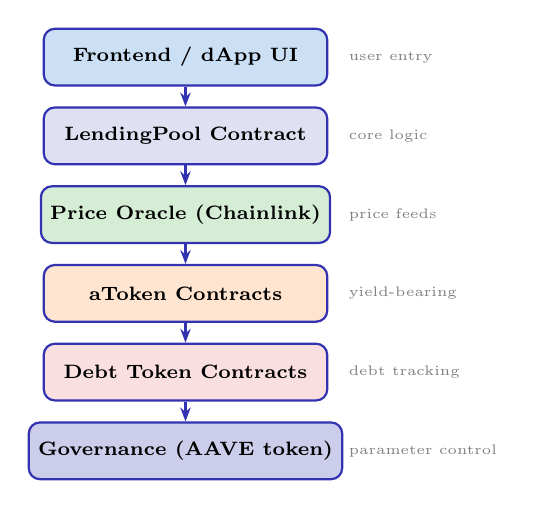
\begin{tikzpicture}[
        compbox/.style={rectangle, rounded corners=4pt, draw=mlpurple, thick,
                        minimum width=3.6cm, minimum height=0.72cm, align=center,
                        font=\scriptsize\bfseries},
        arr/.style={-{Stealth[length=5pt]}, thick, mlpurple}
      ]
        \node[compbox, fill=mlblue!20]    (ui)    at (0, 4.2) {Frontend / dApp UI};
        \node[compbox, fill=mlpurple!15]  (pool)  at (0, 3.2) {LendingPool Contract};
        \node[compbox, fill=mlgreen!20]   (oracle)at (0, 2.2) {Price Oracle (Chainlink)};
        \node[compbox, fill=mlorange!20]  (atoken)at (0, 1.2) {aToken Contracts};
        \node[compbox, fill=mlred!15]     (debt)  at (0, 0.2) {Debt Token Contracts};
        \node[compbox, fill=mllavender3]  (gov)   at (0,-0.8) {Governance (AAVE token)};

        \draw[arr] (ui.south)     -- (pool.north);
        \draw[arr] (pool.south)   -- (oracle.north);
        \draw[arr] (oracle.south) -- (atoken.north);
        \draw[arr] (atoken.south) -- (debt.north);
        \draw[arr] (debt.south)   -- (gov.north);

        \node[font=\tiny, mlgray, anchor=west] at (1.95, 4.2) {user entry};
        \node[font=\tiny, mlgray, anchor=west] at (1.95, 3.2) {core logic};
        \node[font=\tiny, mlgray, anchor=west] at (1.95, 2.2) {price feeds};
        \node[font=\tiny, mlgray, anchor=west] at (1.95, 1.2) {yield-bearing};
        \node[font=\tiny, mlgray, anchor=west] at (1.95, 0.2) {debt tracking};
        \node[font=\tiny, mlgray, anchor=west] at (1.95,-0.8) {parameter control};
      \end{tikzpicture}
    \end{column}
    \begin{column}{0.50\textwidth}
\begin{lstlisting}[language=Solidity, caption={}]
// Simplified Aave Lending Pool
interface ILendingPool {
    // Supply assets to earn interest
    function supply(
        address asset,
        uint256 amount,
        address onBehalfOf
    ) external;

    // Borrow against collateral
    function borrow(
        address asset,
        uint256 amount,
        uint256 interestRateMode  // 1=stable, 2=variable
    ) external;
}
\end{lstlisting}
      \vspace{3mm}
      \begin{block}{aToken Mechanics}
        When you supply 100 DAI, you receive 100 \texttt{aDAI}. The \texttt{aDAI} balance increases
        every block as interest accrues. Redeeming 1 \texttt{aDAI} always yields $\geq 1$ DAI.
      \end{block}
    \end{column}
  \end{columns}
  \bottomnote{Aave's modular architecture separates concerns: core pool logic, oracle pricing, yield tokens, and governance are independent contracts}
\end{frame}

% Frame 35: Compound vs Aave
\begin{frame}{Compound vs.\ Aave: Protocol Comparison}
  \centering
  \adjustbox{max width=\textwidth, max totalheight=6.5cm}{%
  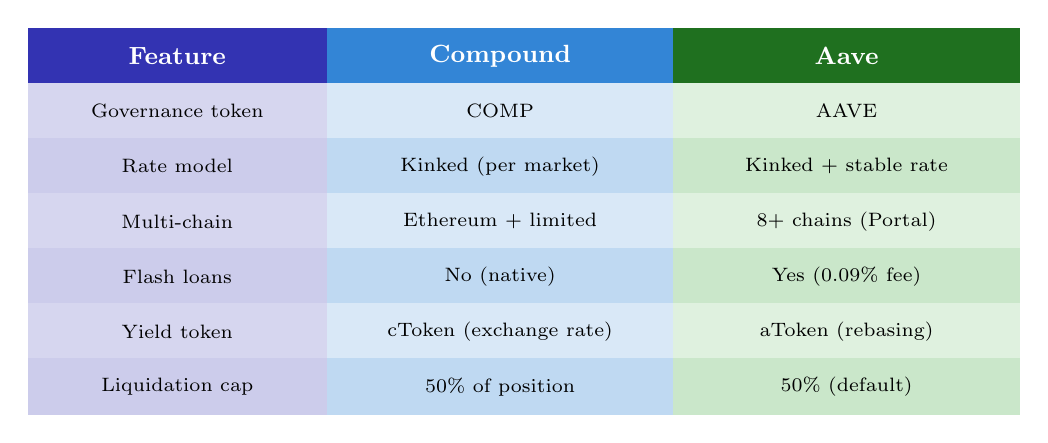
\begin{tikzpicture}[
    hdr/.style={rectangle, minimum height=0.72cm, align=center,
                font=\small\bfseries, text=white},
    celA/.style={rectangle, minimum height=0.72cm, align=center, font=\scriptsize,
                 fill=mlblue!15},
    celB/.style={rectangle, minimum height=0.72cm, align=center, font=\scriptsize,
                 fill=mlgreen!15},
    altA/.style={rectangle, minimum height=0.72cm, align=center, font=\scriptsize,
                 fill=mlblue!25},
    altB/.style={rectangle, minimum height=0.72cm, align=center, font=\scriptsize,
                 fill=mlgreen!25}
  ]
    % Header row
    \node[hdr, minimum width=3.8cm, fill=mlpurple]  at (0,    0) {Feature};
    \node[hdr, minimum width=4.4cm, fill=mlblue!80]  at (4.1,  0) {Compound};
    \node[hdr, minimum width=4.4cm, fill=mlgreen!70!black] at (8.5, 0) {Aave};

    % Row 1: Governance token
    \node[rectangle, fill=mllavender4, minimum height=0.72cm, minimum width=3.8cm,
          align=center, font=\scriptsize] at (0,   -0.7) {Governance token};
    \node[celA, minimum width=4.4cm] at (4.1,  -0.7) {COMP};
    \node[celB, minimum width=4.4cm] at (8.5,  -0.7) {AAVE};

    % Row 2: Interest rate model
    \node[rectangle, fill=mllavender3, minimum height=0.72cm, minimum width=3.8cm,
          align=center, font=\scriptsize] at (0,   -1.4) {Rate model};
    \node[altA, minimum width=4.4cm] at (4.1, -1.4) {Kinked (per market)};
    \node[altB, minimum width=4.4cm] at (8.5, -1.4) {Kinked + stable rate};

    % Row 3: Multi-chain
    \node[rectangle, fill=mllavender4, minimum height=0.72cm, minimum width=3.8cm,
          align=center, font=\scriptsize] at (0,   -2.1) {Multi-chain};
    \node[celA, minimum width=4.4cm] at (4.1,  -2.1) {Ethereum + limited};
    \node[celB, minimum width=4.4cm] at (8.5,  -2.1) {8+ chains (Portal)};

    % Row 4: Flash loans
    \node[rectangle, fill=mllavender3, minimum height=0.72cm, minimum width=3.8cm,
          align=center, font=\scriptsize] at (0,   -2.8) {Flash loans};
    \node[altA, minimum width=4.4cm] at (4.1, -2.8) {No (native)};
    \node[altB, minimum width=4.4cm] at (8.5, -2.8) {Yes (0.09\% fee)};

    % Row 5: Token standard
    \node[rectangle, fill=mllavender4, minimum height=0.72cm, minimum width=3.8cm,
          align=center, font=\scriptsize] at (0,   -3.5) {Yield token};
    \node[celA, minimum width=4.4cm] at (4.1,  -3.5) {cToken (exchange rate)};
    \node[celB, minimum width=4.4cm] at (8.5,  -3.5) {aToken (rebasing)};

    % Row 6: Liquidation
    \node[rectangle, fill=mllavender3, minimum height=0.72cm, minimum width=3.8cm,
          align=center, font=\scriptsize] at (0,   -4.2) {Liquidation cap};
    \node[altA, minimum width=4.4cm] at (4.1, -4.2) {50\% of position};
    \node[altB, minimum width=4.4cm] at (8.5, -4.2) {50\% (default)};
  \end{tikzpicture}
  }%
  \bottomnote{Compound pioneered DeFi lending in 2018; Aave extended the model with stable rates, flash loans, and multi-chain support}
\end{frame}

% Frame 36: Stablecoins in DeFi
\begin{frame}{Stablecoins in DeFi}
  \centering
  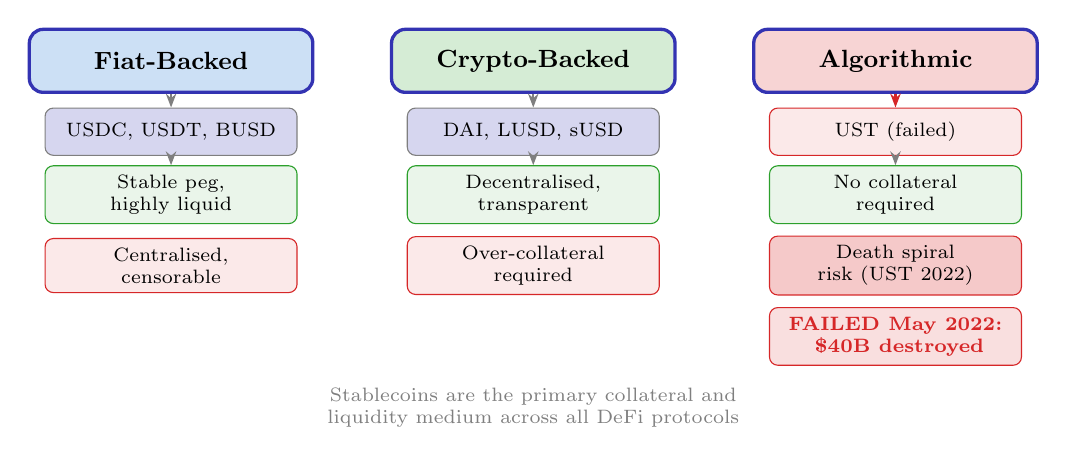
\begin{tikzpicture}[
    catbox/.style={rectangle, rounded corners=5pt, draw=mlpurple, very thick,
                   minimum width=3.6cm, minimum height=0.8cm, align=center,
                   font=\small\bfseries},
    subbox/.style={rectangle, rounded corners=3pt, draw=mlgray, fill=mllavender4,
                   minimum width=3.2cm, minimum height=0.6cm, align=center,
                   font=\scriptsize},
    probox/.style={rectangle, draw=mlgreen, fill=mlgreen!10, rounded corners=3pt,
                   minimum width=3.2cm, minimum height=0.55cm, align=center,
                   font=\scriptsize},
    conbox/.style={rectangle, draw=mlred, fill=mlred!10, rounded corners=3pt,
                   minimum width=3.2cm, minimum height=0.55cm, align=center,
                   font=\scriptsize},
    arr/.style={-{Stealth[length=5pt]}, thick, mlgray}
  ]
    % Category 1: Fiat-backed
    \node[catbox, fill=mlblue!20]   (fb) at (0, 3.0)  {Fiat-Backed};
    \node[subbox] (fbt) at (0, 2.1) {USDC, USDT, BUSD};
    \node[probox] (fbp) at (0, 1.3) {Stable peg,\\highly liquid};
    \node[conbox] (fbc) at (0, 0.4) {Centralised,\\censorable};
    \draw[arr] (fb.south) -- (fbt.north);
    \draw[arr] (fbt.south) -- (fbp.north);

    % Category 2: Crypto-backed
    \node[catbox, fill=mlgreen!20]  (cb) at (4.6, 3.0) {Crypto-Backed};
    \node[subbox] (cbt) at (4.6, 2.1) {DAI, LUSD, sUSD};
    \node[probox] (cbp) at (4.6, 1.3) {Decentralised,\\transparent};
    \node[conbox] (cbc) at (4.6, 0.4) {Over-collateral\\required};
    \draw[arr] (cb.south) -- (cbt.north);
    \draw[arr] (cbt.south) -- (cbp.north);

    % Category 3: Algorithmic (with warning)
    \node[catbox, fill=mlred!20]    (ab) at (9.2, 3.0) {Algorithmic};
    \node[subbox, fill=mlred!10, draw=mlred] (abt) at (9.2, 2.1) {UST (failed)};
    \node[probox] (abp) at (9.2, 1.3) {No collateral\\required};
    \node[conbox, fill=mlred!25] (abc) at (9.2, 0.4) {Death spiral\\risk (UST 2022)};
    \draw[arr, mlred] (ab.south) -- (abt.north);
    \draw[arr] (abt.south) -- (abp.north);

    % Warning box for algorithmic
    \node[rectangle, rounded corners=3pt, draw=mlred, fill=mlred!15,
          minimum width=3.2cm, minimum height=0.65cm, align=center, font=\scriptsize\bfseries,
          text=mlred] at (9.2, -0.5)
      {FAILED May 2022:\\~\$40B destroyed};

    % TVL note
    \node[font=\scriptsize, mlgray, align=center] at (4.6, -1.4)
      {Stablecoins are the primary collateral and\\liquidity medium across all DeFi protocols};
  \end{tikzpicture}
  \bottomnote{Stablecoin choice involves a trust-decentralisation tradeoff; the 2022 Terra/LUNA collapse remains the largest algorithmic failure}
\end{frame}

% Frame 37: MakerDAO and DAI
\begin{frame}{MakerDAO and DAI: Crypto-Backed Stablecoin}
  \begin{columns}[T]
    \begin{column}{0.54\textwidth}
      \centering
      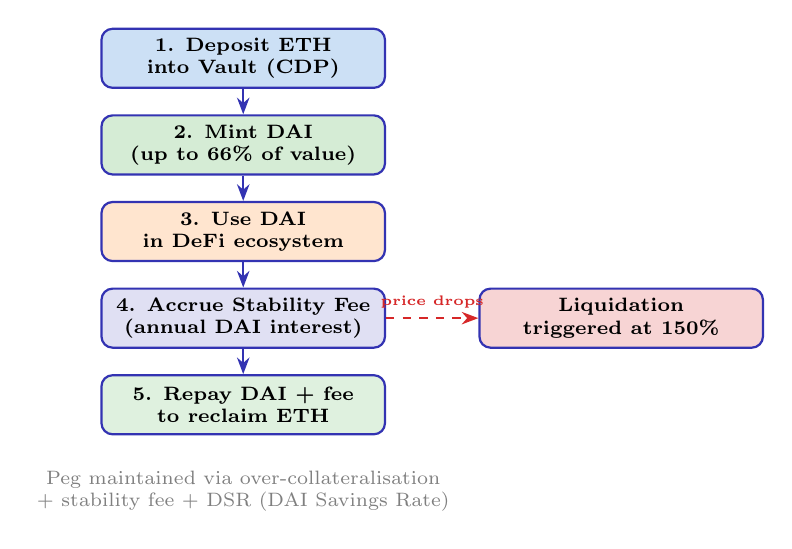
\begin{tikzpicture}[
        procbox/.style={rectangle, rounded corners=4pt, draw=mlpurple, thick,
                        minimum width=3.6cm, minimum height=0.75cm, align=center,
                        font=\scriptsize\bfseries},
        arr/.style={-{Stealth[length=6pt]}, thick}
      ]
        % CDP flow
        \node[procbox, fill=mlblue!20]   (dep)  at (0, 4.0) {1. Deposit ETH\\into Vault (CDP)};
        \node[procbox, fill=mlgreen!20]  (mint) at (0, 2.9) {2. Mint DAI\\(up to 66\% of value)};
        \node[procbox, fill=mlorange!20] (use)  at (0, 1.8) {3. Use DAI\\in DeFi ecosystem};
        \node[procbox, fill=mlpurple!15] (fee)  at (0, 0.7) {4. Accrue Stability Fee\\(annual DAI interest)};
        \node[procbox, fill=mlgreen!15]  (rep)  at (0,-0.4) {5. Repay DAI + fee\\to reclaim ETH};

        \draw[-{Stealth[length=6pt]}, thick, mlpurple] (dep.south)  -- (mint.north);
        \draw[-{Stealth[length=6pt]}, thick, mlpurple] (mint.south) -- (use.north);
        \draw[-{Stealth[length=6pt]}, thick, mlpurple] (use.south)  -- (fee.north);
        \draw[-{Stealth[length=6pt]}, thick, mlpurple] (fee.south)  -- (rep.north);

        % Liquidation branch
        \node[procbox, fill=mlred!20] (liq) at (4.8, 0.7) {Liquidation\\triggered at 150\%};
        \draw[-{Stealth[length=6pt]}, thick, mlred, dashed] (fee.east) -- (liq.west)
          node[midway, above, font=\tiny\bfseries, mlred] {price drops};

        % Peg mechanism
        \node[font=\scriptsize, mlgray, align=center] at (0,-1.5)
          {Peg maintained via over-collateralisation\\+ stability fee + DSR (DAI Savings Rate)};
      \end{tikzpicture}
    \end{column}
    \begin{column}{0.42\textwidth}
      \begin{block}{Key Parameters}
        \begin{tabular}{ll}
          \toprule
          Parameter & Value \\
          \midrule
          Min collateral ratio & 150\% \\
          Liquidation penalty  & 13\%  \\
          Stability fee (APR)  & 0--10\% (variable) \\
          DAI Savings Rate     & governance-set \\
          \bottomrule
        \end{tabular}
      \end{block}
      \vspace{1mm}
      \begin{block}{Peg Stability Mechanisms}
        \begin{itemize}\setlength\itemsep{1pt}
          \item \textbf{Over-collateralisation} ensures DAI is always backed
          \item \textbf{Stability fee} controls minting incentive (DAI supply)
          \item \textbf{DSR} controls holding incentive (DAI demand)
          \item \textbf{PSM} (Peg Stability Module) allows 1:1 USDC swap at zero fee
        \end{itemize}
      \end{block}
      \vspace{1mm}
      \begin{alertblock}{Multi-Collateral DAI}
        MakerDAO expanded to accept 40+ collateral types including real-world assets (RWA),
        making DAI partially dependent on centralised assets.
      \end{alertblock}
    \end{column}
  \end{columns}
  \bottomnote{MakerDAO launched in 2017 and remains the leading decentralised stablecoin protocol; DAI is the dominant non-custodial stablecoin}
\end{frame}

% Frame 38: Section 3 Summary
\begin{frame}{Section 3 Summary: Lending and Borrowing}
  \begin{columns}[T]
    \begin{column}{0.48\textwidth}
      \begin{block}{Key Takeaways}
        \begin{enumerate}\setlength\itemsep{4pt}
          \item \textbf{DeFi lending} is permissionless and overcollateralised: borrowers lock
                crypto collateral to access liquidity without credit checks
          \item \textbf{Kinked interest rate models} dynamically price credit by utilisation rate,
                automatically incentivising liquidity at both extremes
          \item \textbf{Liquidation} is the protocol's solvency backstop: unhealthy positions are
                closed by profit-seeking liquidators who repay debt and claim collateral at a discount
          \item \textbf{Health factor} aggregates multi-asset collateral with asset-specific
                liquidation thresholds into a single solvency signal
          \item \textbf{Stablecoins} --- fiat-backed, crypto-backed, and algorithmic --- each carry
                distinct trust assumptions and failure modes
        \end{enumerate}
      \end{block}
    \end{column}
    \begin{column}{0.48\textwidth}
      \begin{block}{Formulas to Remember}
        \[
          HF = \frac{\sum_i V_{c,i} \cdot LT_i}{V_{\text{debt,total}}}
        \]
        \[
          r(U) = r_{\text{base}} + \frac{U}{U^*} s_1 \quad (U \leq U^*)
        \]
        \[
          r(U) = r_{\text{base}} + s_1 + \frac{U - U^*}{1 - U^*} s_2 \quad (U > U^*)
        \]
        \[
          CR = \frac{V_{\text{collateral}}}{V_{\text{debt}}} \geq CR_{\min}
        \]
      \end{block}
      \vspace{3mm}
      \begin{alertblock}{Coming Up: Section 4}
        Yield Farming --- liquidity mining, token emissions, APY calculation, and impermanent loss
        under incentivised pools.
      \end{alertblock}
    \end{column}
  \end{columns}
  \bottomnote{Section 3 complete | Next: Section 4 --- Yield Farming | Frames 39 onward}
\end{frame}

%% ============================================================
%% SECTION 4: YIELD FARMING & LIQUIDITY MINING
%% ============================================================

\section{Yield Farming \& Liquidity Mining}

% Frame 39: Section Divider
\begin{frame}
  \begin{beamercolorbox}[sep=12pt,center,rounded=true,shadow=true]{palette quaternary}
    {\Large\bfseries Section 4: Yield Farming and Liquidity Mining}\\{}\vspace{6pt}
    {\normalsize LP tokens, APR vs APY, impermanent loss, yield strategies, and real yield analysis}
  \end{beamercolorbox}
  \vspace{8mm}
  \begin{columns}[T]
    \begin{column}{0.48\textwidth}
      \begin{block}{What you will learn}
        \begin{itemize}\setlength\itemsep{2pt}
          \item What is yield farming?
          \item LP token mechanics
          \item APR vs APY calculations
          \item Impermanent loss in practice
          \item Yield farming strategies
          \item Real yield vs token emissions
          \item Yield aggregators (Yearn)
        \end{itemize}
      \end{block}
    \end{column}
    \begin{column}{0.48\textwidth}
      \begin{block}{Frames in this section}
        \begin{itemize}\setlength\itemsep{2pt}
          \item Frame 40 -- What is Yield Farming?
          \item Frame 41 -- LP Token Mechanics
          \item Frames 42--43 -- APR vs APY, Compounding
          \item Frames 44--45 -- Impermanent Loss, Strategies
          \item Frames 46--48 -- Real Yield, Aggregators, Summary
        \end{itemize}
      \end{block}
    \end{column}
  \end{columns}
  \bottomnote{Section 4 of 5 | Yield Farming \& Liquidity Mining | Frames 39--48}
\end{frame}

% Frame 40: What is Yield Farming?
\begin{frame}{What is Yield Farming?}
  \begin{center}
  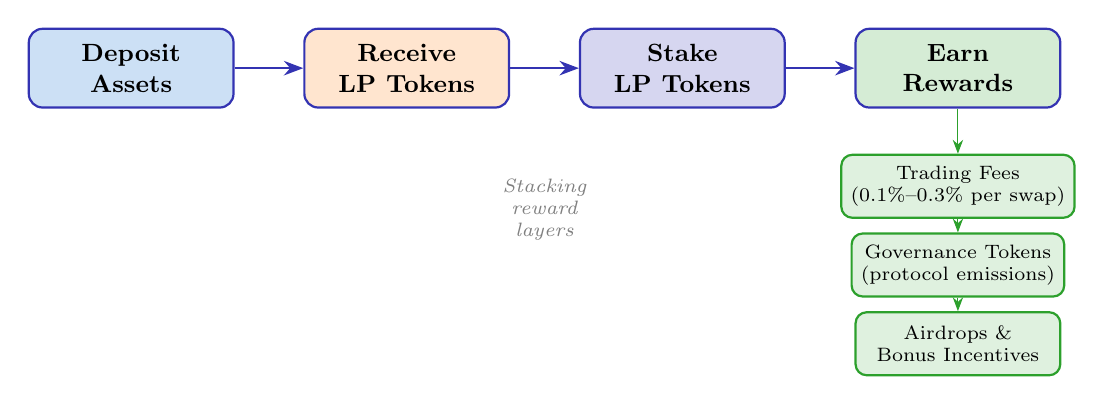
\begin{tikzpicture}[
    box/.style={rectangle, rounded corners=5pt, minimum width=2.6cm, minimum height=1.0cm,
      draw=mlpurple, thick, align=center, font=\small\bfseries},
    reward/.style={rectangle, rounded corners=4pt, minimum width=2.6cm, minimum height=0.8cm,
      draw=mlgreen, thick, fill=mlgreen!15, align=center, font=\scriptsize}
  ]
    % Main flow row
    \node[box, fill=mlblue!20]    (dep)   at (0,0)   {Deposit\\Assets};
    \node[box, fill=mlorange!20]  (lp)    at (3.5,0)  {Receive\\LP Tokens};
    \node[box, fill=mlpurple!20]  (stake) at (7.0,0)  {Stake\\LP Tokens};
    \node[box, fill=mlgreen!20]   (earn)  at (10.5,0) {Earn\\Rewards};

    \draw[-{Stealth[length=7pt]}, thick, mlpurple] (dep.east)   -- (lp.west);
    \draw[-{Stealth[length=7pt]}, thick, mlpurple] (lp.east)    -- (stake.west);
    \draw[-{Stealth[length=7pt]}, thick, mlpurple] (stake.east) -- (earn.west);

    % Reward layers beneath earn
    \node[reward] (r1) at (10.5,-1.5) {Trading Fees\\(0.1\%--0.3\% per swap)};
    \node[reward] (r2) at (10.5,-2.5) {Governance Tokens\\(protocol emissions)};
    \node[reward] (r3) at (10.5,-3.5) {Airdrops \&\\Bonus Incentives};

    \draw[-{Stealth[length=5pt]}, mlgreen] (earn.south) -- (r1.north);
    \draw[-{Stealth[length=5pt]}, mlgreen] (r1.south)   -- (r2.north);
    \draw[-{Stealth[length=5pt]}, mlgreen] (r2.south)   -- (r3.north);

    % Label
    \node[font=\scriptsize\itshape, text=mlgray, align=center] at (5.25, -1.8) {Stacking\\reward\\layers};
  \end{tikzpicture}
  \end{center}
  \vspace{2mm}
  \begin{block}{Definition}
    \textbf{Yield farming} is the practice of deploying crypto assets into DeFi protocols
    to generate returns from multiple stacked incentive layers simultaneously.
    Farmers optimise across protocols seeking the highest risk-adjusted yield.
  \end{block}
  \bottomnote{Yield farming = deposit + stake + earn; rewards stack across fees, governance tokens, and airdrops}
\end{frame}

% Frame 41: LP Token Mechanics
\begin{frame}{LP Token Mechanics}
  \begin{columns}[T]
    \begin{column}{0.52\textwidth}
      \begin{center}
      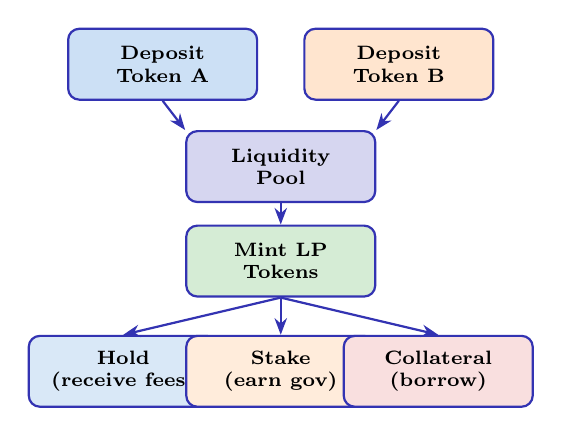
\begin{tikzpicture}[
        box/.style={rectangle, rounded corners=4pt, minimum width=2.4cm, minimum height=0.9cm,
          draw=mlpurple, thick, align=center, font=\scriptsize\bfseries},
        arrow/.style={-{Stealth[length=6pt]}, thick, mlpurple}
      ]
        \node[box, fill=mlblue!20]   (a) at (0,2.5)   {Deposit\\Token A};
        \node[box, fill=mlorange!20] (b) at (3,2.5)   {Deposit\\Token B};
        \node[box, fill=mlpurple!20] (pool) at (1.5,1.2) {Liquidity\\Pool};
        \node[box, fill=mlgreen!20]  (lp) at (1.5,0)  {Mint LP\\Tokens};
        \node[box, fill=mlblue!15]   (hold) at (-0.5,-1.4) {Hold\\(receive fees)};
        \node[box, fill=mlorange!15] (stk)  at (1.5,-1.4)  {Stake\\(earn gov)};
        \node[box, fill=mlred!15]    (col)  at (3.5,-1.4)  {Collateral\\(borrow)};

        \draw[arrow] (a.south)    -- (pool.north west);
        \draw[arrow] (b.south)    -- (pool.north east);
        \draw[arrow] (pool.south) -- (lp.north);
        \draw[arrow] (lp.south)   -- (hold.north);
        \draw[arrow] (lp.south)   -- (stk.north);
        \draw[arrow] (lp.south)   -- (col.north);
      \end{tikzpicture}
      \end{center}
    \end{column}
    \begin{column}{0.45\textwidth}
      \begin{block}{LP Token Formula}
        \vspace{2mm}
        For a constant-product pool:
        \[
          \text{LP}_{\text{minted}} = \sqrt{x \cdot y}
        \]
        where $x$ = amount of Token A deposited, $y$ = amount of Token B deposited.

        \vspace{3mm}
        \textbf{Redemption share:}
        \[
          \text{share} = \frac{\text{LP}_{\text{held}}}{\text{LP}_{\text{total}}}
        \]
        You withdraw \texttt{share} $\times$ pool balance of each token.
      \end{block}
      \begin{alertblock}{Key Property}
        LP tokens are composable --- they can be staked, used as collateral,
        or bridged, enabling nested yield strategies.
      \end{alertblock}
    \end{column}
  \end{columns}
  \bottomnote{LP tokens represent proportional pool ownership; formula: $\sqrt{A \times B}$; composable across DeFi protocols}
\end{frame}

% Frame 42: APR vs APY
\begin{frame}{APR vs APY}
  \begin{columns}[T]
    \begin{column}{0.44\textwidth}
      \begin{block}{Definitions}
        \textbf{APR} --- Annual Percentage Rate (simple, no compounding):
        \[ \text{APR} = r \times n \]

        \textbf{APY} --- Annual Percentage Yield (with compounding $n$ times/year):
        \[
          \text{APY} = \left(1 + \frac{\text{APR}}{n}\right)^{n} - 1
        \]
      \end{block}
      \begin{block}{Example: 50\% APR}
        \begin{itemize}\setlength\itemsep{2pt}
          \item Weekly ($n=52$): APY $= 64.5\%$
          \item Daily ($n=365$): APY $= 64.8\%$
          \item Hourly ($n=8760$): APY $= 64.87\%$
          \item Continuous: APY $= e^{0.5}-1 = 64.87\%$
        \end{itemize}
        \textit{Gap grows dramatically at high APR.}
      \end{block}
    \end{column}
    \begin{column}{0.53\textwidth}
      \begin{center}
      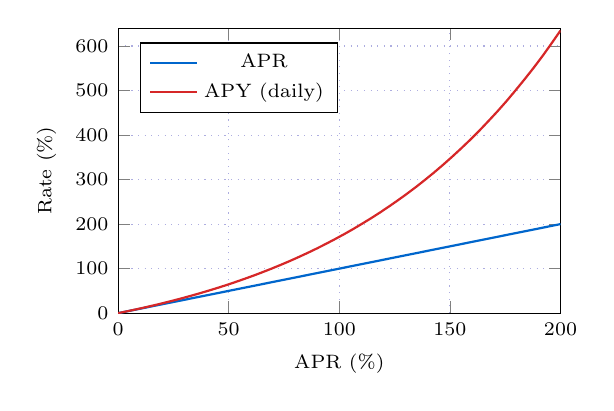
\begin{tikzpicture}
        \begin{axis}[
          width=7.2cm, height=5.2cm,
          xlabel={APR (\%)}, ylabel={Rate (\%)},
          xmin=0, xmax=200, ymin=0, ymax=640,
          xtick={0,50,100,150,200},
          ytick={0,100,200,300,400,500,600},
          grid=major, grid style={dotted, mllavender},
          tick label style={font=\scriptsize},
          label style={font=\scriptsize},
          legend style={font=\scriptsize, at={(0.05,0.95)}, anchor=north west}
        ]
          % APR line (identity)
          \addplot[thick, mlblue, domain=0:200, samples=50] {x};
          \addlegendentry{APR}
          % APY daily compounding: (1+x/36500)^365 - 1 * 100, x in percent
          \addplot[thick, mlred, domain=0:200, samples=50]
            {(((1 + x/36500)^365) - 1)*100};
          \addlegendentry{APY (daily)}
        \end{axis}
      \end{tikzpicture}
      \end{center}
      \begin{alertblock}{Warning}
        DeFi protocols advertise APY, but token emissions may decline --- actual returns
        are lower than headline figures suggest.
      \end{alertblock}
    \end{column}
  \end{columns}
  \bottomnote{APY $=(1+\text{APR}/n)^n -1$; divergence accelerates above 100\% APR; always check emission schedules}
\end{frame}

% Frame 43: Impermanent Loss in Practice
\begin{frame}{Impermanent Loss in Practice}
  \begin{columns}[T]
    \begin{column}{0.50\textwidth}
      \begin{block}{Real Scenario}
        \textbf{Initial deposit:}
        \begin{itemize}\setlength\itemsep{1pt}
          \item 1 ETH at \$2{,}000 + 2{,}000 USDC
          \item Total value: \$4{,}000
          \item $k = 1 \times 2000 = 2000$
        \end{itemize}

        \vspace{2mm}
        \textbf{ETH price rises to \$4{,}000:}
        \begin{itemize}\setlength\itemsep{1pt}
          \item New pool state: $\sqrt{2000/4000} \approx 0.707$ ETH, $2828$ USDC
          \item Pool value: $0.707 \times 4000 + 2828 = \$5{,}656$
          \item \textit{Without LP}: $1 \times 4000 + 2000 = \$6{,}000$
        \end{itemize}

        \vspace{2mm}
        \begin{alertblock}{Impermanent Loss}
          \[
            \text{IL} = \frac{5656 - 6000}{6000} \approx -5.7\%
          \]
          You hold \textit{less} of the appreciating asset.
        \end{alertblock}
      \end{block}
    \end{column}
    \begin{column}{0.47\textwidth}
      \begin{center}
      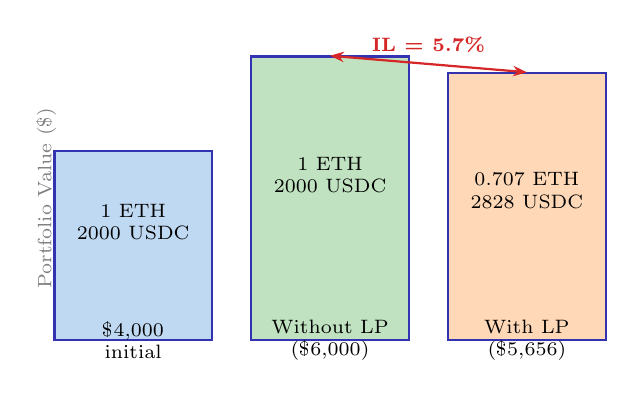
\begin{tikzpicture}[
        bar/.style={rectangle, minimum width=2.0cm, draw=mlpurple, thick},
        lbl/.style={font=\scriptsize, align=center}
      ]
        % Before bar
        \node[bar, minimum height=2.4cm, fill=mlblue!25]  (bef) at (0,1.2)  {};
        \node[lbl] at (0,0)    {\$4{,}000\\initial};
        \node[lbl, font=\scriptsize] at (0,1.5) {1 ETH\\2000 USDC};

        % Without LP bar
        \node[bar, minimum height=3.6cm, fill=mlgreen!30] (wol) at (2.5,1.8) {};
        \node[lbl] at (2.5,0)   {Without LP\\(\$6{,}000)};
        \node[lbl, font=\scriptsize] at (2.5,2.1) {1 ETH\\2000 USDC};

        % With LP bar
        \node[bar, minimum height=3.39cm, fill=mlorange!30] (wlp) at (5.0,1.695) {};
        \node[lbl] at (5.0,0)   {With LP\\(\$5{,}656)};
        \node[lbl, font=\scriptsize] at (5.0,1.9) {0.707 ETH\\2828 USDC};

        % IL annotation
        \draw[{Stealth[length=5pt]}-{Stealth[length=5pt]}, thick, mlred]
          (2.5,3.61) -- (5.0,3.40);
        \node[font=\scriptsize\bfseries, text=mlred] at (3.75,3.75) {IL = 5.7\%};

        % y-axis label
        \node[font=\scriptsize, rotate=90, text=mlgray] at (-1.1,1.8) {Portfolio Value (\$)};
      \end{tikzpicture}
      \end{center}
    \end{column}
  \end{columns}
  \bottomnote{IL formula: $\frac{2\sqrt{r}}{1+r}-1$ where $r$ = price ratio; IL is temporary only if prices revert}
\end{frame}

% Frame 44: Impermanent Loss Table
\begin{frame}{Impermanent Loss Table}
  \vspace{1mm}
  \begin{center}
  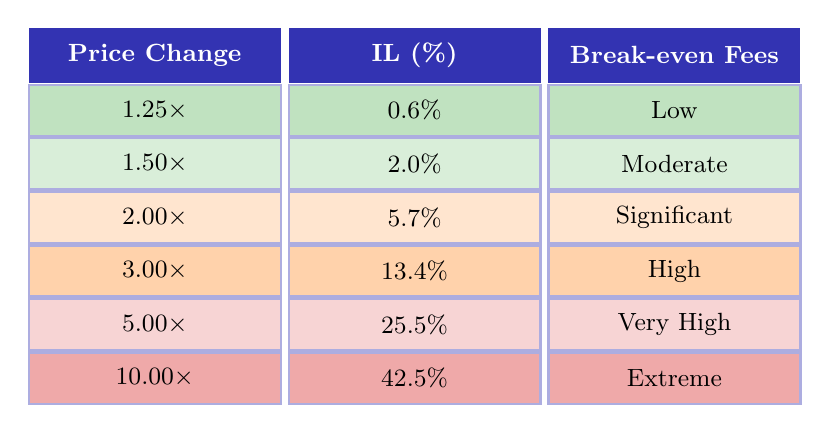
\begin{tikzpicture}[
    hdr/.style={rectangle, minimum width=3.2cm, minimum height=0.7cm,
      fill=mlpurple, text=white, font=\small\bfseries, align=center},
    cel/.style={rectangle, minimum width=3.2cm, minimum height=0.65cm,
      draw=mllavender, thick, align=center, font=\small}
  ]
    % Headers
    \node[hdr] (h1) at (0,0)    {Price Change};
    \node[hdr] (h2) at (3.3,0)  {IL (\%)};
    \node[hdr] (h3) at (6.6,0)  {Break-even Fees};

    % Row 1 -- near green
    \node[cel, fill=mlgreen!30]  at (0,-0.70)   {1.25$\times$};
    \node[cel, fill=mlgreen!30]  at (3.3,-0.70)  {0.6\%};
    \node[cel, fill=mlgreen!30]  at (6.6,-0.70)  {Low};

    % Row 2
    \node[cel, fill=mlgreen!18]  at (0,-1.38)   {1.50$\times$};
    \node[cel, fill=mlgreen!18]  at (3.3,-1.38)  {2.0\%};
    \node[cel, fill=mlgreen!18]  at (6.6,-1.38)  {Moderate};

    % Row 3
    \node[cel, fill=mlorange!20] at (0,-2.06)   {2.00$\times$};
    \node[cel, fill=mlorange!20] at (3.3,-2.06)  {5.7\%};
    \node[cel, fill=mlorange!20] at (6.6,-2.06)  {Significant};

    % Row 4
    \node[cel, fill=mlorange!35] at (0,-2.74)   {3.00$\times$};
    \node[cel, fill=mlorange!35] at (3.3,-2.74)  {13.4\%};
    \node[cel, fill=mlorange!35] at (6.6,-2.74)  {High};

    % Row 5
    \node[cel, fill=mlred!20]    at (0,-3.42)   {5.00$\times$};
    \node[cel, fill=mlred!20]    at (3.3,-3.42)  {25.5\%};
    \node[cel, fill=mlred!20]    at (6.6,-3.42)  {Very High};

    % Row 6 -- deepest red
    \node[cel, fill=mlred!40]    at (0,-4.10)   {10.00$\times$};
    \node[cel, fill=mlred!40]    at (3.3,-4.10)  {42.5\%};
    \node[cel, fill=mlred!40]    at (6.6,-4.10)  {Extreme};
  \end{tikzpicture}
  \end{center}
  \vspace{2mm}
  \begin{block}{IL Formula}
    \[
      \text{IL}(r) = \frac{2\sqrt{r}}{1+r} - 1, \quad r = \frac{P_{\text{new}}}{P_{\text{initial}}}
    \]
    IL is \emph{permanent} if you withdraw when prices diverge; fees must exceed IL to be profitable.
  \end{block}
  \bottomnote{IL grows super-linearly with price change; stable-pair pools (r$\approx$1) have near-zero IL}
\end{frame}

% Frame 45: Yield Farming Strategies
\begin{frame}{Yield Farming Strategies}
  \begin{center}
  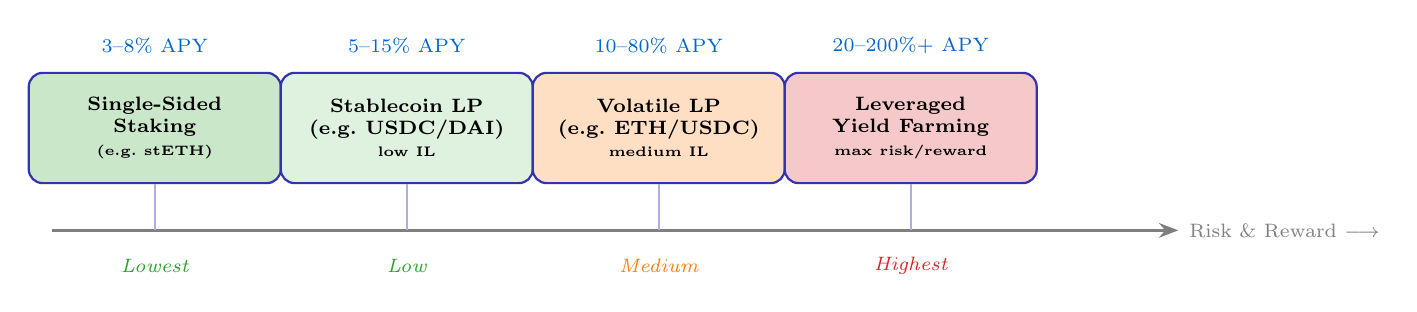
\begin{tikzpicture}[
    strat/.style={rectangle, rounded corners=5pt, minimum width=3.2cm, minimum height=1.4cm,
      draw=mlpurple, thick, align=center, font=\scriptsize\bfseries},
    axis/.style={-{Stealth[length=7pt]}, very thick, mlgray}
  ]
    % Risk/Reward axis
    \draw[axis] (-0.5,-0.1) -- (13.8,-0.1) node[right, font=\scriptsize] {Risk \& Reward $\longrightarrow$};

    % Strategy boxes along axis
    \node[strat, fill=mlgreen!25]   (s1) at (0.8,1.2)  {Single-Sided\\Staking\\{\tiny (e.g.\ stETH)}};
    \node[strat, fill=mlgreen!15]   (s2) at (4.0,1.2)  {Stablecoin LP\\(e.g.\ USDC/DAI)\\{\tiny low IL}};
    \node[strat, fill=mlorange!25]  (s3) at (7.2,1.2)  {Volatile LP\\(e.g.\ ETH/USDC)\\{\tiny medium IL}};
    \node[strat, fill=mlred!25]     (s4) at (10.4,1.2) {Leveraged\\Yield Farming\\{\tiny max risk/reward}};

    % Connectors to axis
    \draw[thick, mllavender] (s1.south) -- (0.8,-0.1);
    \draw[thick, mllavender] (s2.south) -- (4.0,-0.1);
    \draw[thick, mllavender] (s3.south) -- (7.2,-0.1);
    \draw[thick, mllavender] (s4.south) -- (10.4,-0.1);

    % Risk labels
    \node[font=\scriptsize\itshape, text=mlgreen]  at (0.8,-0.55)  {Lowest};
    \node[font=\scriptsize\itshape, text=mlgreen]  at (4.0,-0.55)  {Low};
    \node[font=\scriptsize\itshape, text=mlorange] at (7.2,-0.55)  {Medium};
    \node[font=\scriptsize\itshape, text=mlred]    at (10.4,-0.55) {Highest};

    % Typical APY labels
    \node[font=\scriptsize, text=mlblue] at (0.8,2.25)  {3--8\% APY};
    \node[font=\scriptsize, text=mlblue] at (4.0,2.25)  {5--15\% APY};
    \node[font=\scriptsize, text=mlblue] at (7.2,2.25)  {10--80\% APY};
    \node[font=\scriptsize, text=mlblue] at (10.4,2.25) {20--200\%+ APY};
  \end{tikzpicture}
  \end{center}
  \vspace{2mm}
  \begin{block}{Strategy Selection Principle}
    Match strategy to risk tolerance. Leveraged farming amplifies IL and liquidation risk;
    stablecoin pools sacrifice upside for consistency. \emph{Higher APY always implies
    higher risk.}
  \end{block}
  \bottomnote{Strategy spectrum: single-sided (safest) $\to$ stablecoin LP $\to$ volatile LP $\to$ leveraged (highest risk)}
\end{frame}

% Frame 46: Real Yield vs Token Emissions
\begin{frame}{Real Yield vs Token Emissions}
  \begin{columns}[T]
    \begin{column}{0.48\textwidth}
      \begin{block}{Real Yield}
        \textbf{Source:} Protocol revenue (trading fees, liquidation fees, interest spreads).

        \vspace{2mm}
        \textbf{Properties:}
        \begin{itemize}\setlength\itemsep{2pt}
          \item Sustainable long-term
          \item Denominated in established tokens (ETH, stables)
          \item Grows with protocol usage
          \item Examples: GMX, dYdX, Curve (3CRV fees)
        \end{itemize}
      \end{block}
      \begin{alertblock}{Evaluation}
        Always compute: \textbf{Real Yield} = Total APY $-$ Emission APY.
        If real yield is near zero, the protocol subsidises LPs unsustainably.
      \end{alertblock}
    \end{column}
    \begin{column}{0.48\textwidth}
      \begin{block}{Token Emissions}
        \textbf{Source:} Protocol mints new governance tokens for LPs.

        \vspace{2mm}
        \textbf{Properties:}
        \begin{itemize}\setlength\itemsep{2pt}
          \item Inflationary by design
          \item Token value may decline faster than yield accrues
          \item Mercenary capital: LPs exit when emissions end
          \item Examples: early Sushiswap, OlympusDAO forks
        \end{itemize}
      \end{block}
      \begin{center}
      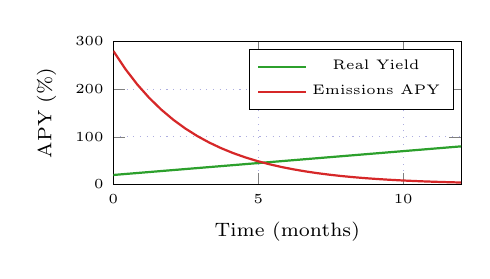
\begin{tikzpicture}
        \begin{axis}[
          width=6.0cm, height=3.4cm,
          xlabel={Time (months)}, ylabel={APY (\%)},
          xmin=0, xmax=12, ymin=0, ymax=300,
          grid=major, grid style={dotted, mllavender},
          tick label style={font=\tiny},
          label style={font=\scriptsize},
          legend style={font=\tiny, at={(0.98,0.95)}, anchor=north east}
        ]
          \addplot[thick, mlgreen, domain=0:12, samples=30] {20 + 5*x};
          \addlegendentry{Real Yield}
          \addplot[thick, mlred, domain=0:12, samples=30] {280*exp(-0.35*x)};
          \addlegendentry{Emissions APY}
        \end{axis}
      \end{tikzpicture}
      \end{center}
    \end{column}
  \end{columns}
  \bottomnote{Real yield = fee revenue; token emissions are inflationary subsidies; distinguish before committing capital}
\end{frame}

% Frame 47: Yield Aggregators
\begin{frame}{Yield Aggregators (e.g.\ Yearn Finance)}
  \begin{columns}[T]
    \begin{column}{0.55\textwidth}
      \begin{center}
      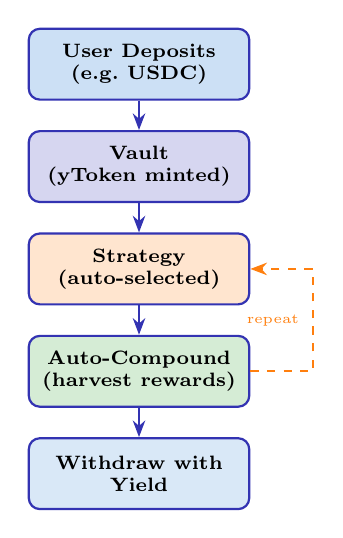
\begin{tikzpicture}[
        box/.style={rectangle, rounded corners=4pt, minimum width=2.8cm, minimum height=0.9cm,
          draw=mlpurple, thick, align=center, font=\scriptsize\bfseries},
        arr/.style={-{Stealth[length=6pt]}, thick, mlpurple}
      ]
        \node[box, fill=mlblue!20]   (usr)   at (0,4.5)  {User Deposits\\(e.g.\ USDC)};
        \node[box, fill=mlpurple!20] (vault) at (0,3.2)  {Vault\\(yToken minted)};
        \node[box, fill=mlorange!20] (strat) at (0,1.9)  {Strategy\\(auto-selected)};
        \node[box, fill=mlgreen!20]  (comp)  at (0,0.6)  {Auto-Compound\\(harvest rewards)};
        \node[box, fill=mlblue!15]   (with)  at (0,-0.7) {Withdraw with\\Yield};

        \draw[arr] (usr.south)   -- (vault.north);
        \draw[arr] (vault.south) -- (strat.north);
        \draw[arr] (strat.south) -- (comp.north);
        \draw[arr] (comp.south)  -- (with.north);

        % Cycle arrow back to strategy
        \draw[arr, dashed, mlorange] (comp.east) -- ++(0.8,0) |-  (strat.east);
        \node[font=\tiny, text=mlorange] at (1.7,1.25) {repeat};
      \end{tikzpicture}
      \end{center}
    \end{column}
    \begin{column}{0.42\textwidth}
      \begin{block}{Benefits of Aggregators}
        \begin{itemize}\setlength\itemsep{3pt}
          \item \textbf{Gas savings}: Socialised harvest costs across many depositors
          \item \textbf{Strategy expertise}: Professionals manage complex DeFi positions
          \item \textbf{Auto-compounding}: Rewards reinvested without manual action
          \item \textbf{Diversification}: Vault can rotate among strategies
          \item \textbf{Risk management}: Strategies audited; loss limits enforced
        \end{itemize}
      \end{block}
      \begin{alertblock}{Cost}
        Performance fee (typically 20\%) on yields.
        Smart contract and strategy risk remain.
      \end{alertblock}
    \end{column}
  \end{columns}
  \bottomnote{Yearn pattern: deposit $\to$ vault $\to$ strategy $\to$ auto-compound; socialises gas and expertise costs}
\end{frame}

% Frame 48: Section 4 Summary
\begin{frame}{Section 4 Summary}
  \vspace{1mm}
  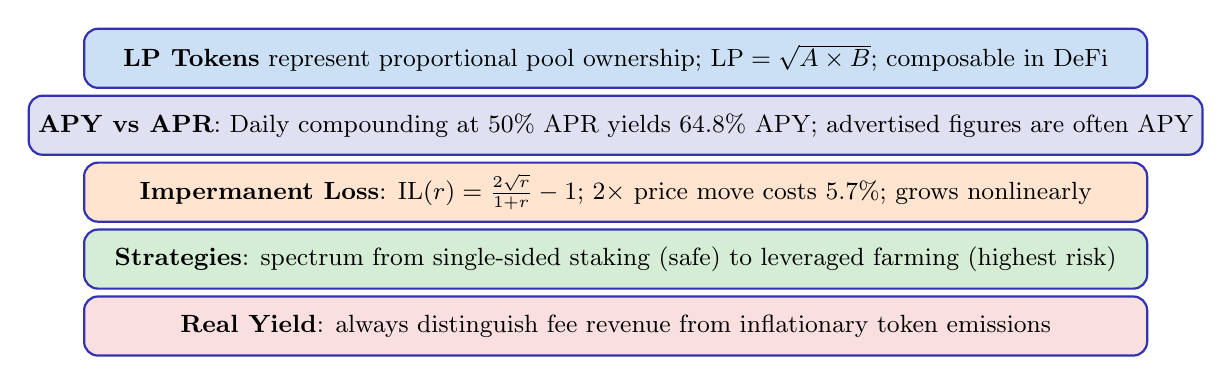
\begin{tikzpicture}[
    sumbox/.style={rectangle, rounded corners=5pt, minimum width=13.5cm, minimum height=0.75cm,
      draw=mlpurple, thick, align=center, font=\small}
  ]
    \node[sumbox, fill=mlblue!20]    at (0,0)    {\textbf{LP Tokens} represent proportional pool ownership; $\text{LP} = \sqrt{A \times B}$; composable in DeFi};
    \node[sumbox, fill=mlpurple!15]  at (0,-0.85) {\textbf{APY vs APR}: Daily compounding at 50\% APR yields 64.8\% APY; advertised figures are often APY};
    \node[sumbox, fill=mlorange!20]  at (0,-1.70) {\textbf{Impermanent Loss}: $\text{IL}(r)=\frac{2\sqrt{r}}{1+r}-1$; 2$\times$ price move costs 5.7\%; grows nonlinearly};
    \node[sumbox, fill=mlgreen!20]   at (0,-2.55) {\textbf{Strategies}: spectrum from single-sided staking (safe) to leveraged farming (highest risk)};
    \node[sumbox, fill=mlred!15]     at (0,-3.40) {\textbf{Real Yield}: always distinguish fee revenue from inflationary token emissions};
  \end{tikzpicture}
  \vspace{2mm}
  \begin{alertblock}{Key Insight}
    Headline APYs combine fees, emissions, and compounding. Decompose each component and
    account for IL before comparing yield farming opportunities.
  \end{alertblock}
  \bottomnote{Section 4 complete | Next: Section 5 --- Advanced Topics | Frames 49--55}
\end{frame}

%% ============================================================
%% SECTION 5: ADVANCED TOPICS & SUMMARY
%% ============================================================

\section{Advanced Topics \& Summary}

% Frame 49: Section Divider
\begin{frame}
  \begin{beamercolorbox}[sep=12pt,center,rounded=true,shadow=true]{palette quaternary}
    {\Large\bfseries Section 5: Advanced Topics and Summary}\\{}\vspace{6pt}
    {\normalsize Flash loans, MEV, DeFi security, attack anatomy, regulation, and course summary}
  \end{beamercolorbox}
  \vspace{8mm}
  \begin{columns}[T]
    \begin{column}{0.48\textwidth}
      \begin{block}{What you will learn}
        \begin{itemize}\setlength\itemsep{2pt}
          \item Flash loans
          \item MEV --- Maximal Extractable Value
          \item DeFi security best practices
          \item Flash loan attack anatomy
          \item Regulatory landscape
          \item Course summary and key takeaways
        \end{itemize}
      \end{block}
    \end{column}
    \begin{column}{0.48\textwidth}
      \begin{block}{Frames in this section}
        \begin{itemize}\setlength\itemsep{2pt}
          \item Frame 50 -- Flash Loans
          \item Frame 51 -- MEV
          \item Frame 52 -- DeFi Security Best Practices
          \item Frames 53--54 -- Flash Loan Attacks, Regulation
          \item Frame 55 -- Key Takeaways and Course Summary
        \end{itemize}
      \end{block}
    \end{column}
  \end{columns}
  \bottomnote{Section 5 of 5 | Advanced Topics \& Summary | Frames 49--55}
\end{frame}

% Frame 50: Flash Loans [FRAGILE]
\begin{frame}[fragile]{Flash Loans}
  \begin{columns}[T]
    \begin{column}{0.44\textwidth}
      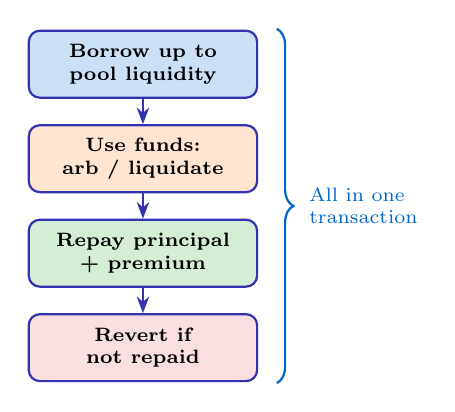
\begin{tikzpicture}[
        box/.style={rectangle, rounded corners=4pt, minimum width=2.9cm, minimum height=0.85cm,
          draw=mlpurple, thick, align=center, font=\scriptsize\bfseries},
        arr/.style={-{Stealth[length=6pt]}, thick, mlpurple}
      ]
        \node[box, fill=mlblue!20]   (bor)  at (0,4.2)  {Borrow up to\\pool liquidity};
        \node[box, fill=mlorange!20] (use)  at (0,3.0)  {Use funds:\\arb / liquidate};
        \node[box, fill=mlgreen!20]  (rep)  at (0,1.8)  {Repay principal\\+ premium};
        \node[box, fill=mlred!15]    (rev)  at (0,0.6)  {Revert if\\not repaid};

        \draw[arr] (bor.south) -- (use.north);
        \draw[arr] (use.south) -- (rep.north);
        \draw[arr] (rep.south) -- (rev.north);

        % Single transaction bracket
        \draw[thick, mlblue, decorate, decoration={brace, amplitude=6pt}]
          (1.7,4.65) -- (1.7,0.15) node[midway, right=8pt, font=\scriptsize, text=mlblue, align=left]
          {All in one\\transaction};
      \end{tikzpicture}
    \end{column}
    \begin{column}{0.54\textwidth}
      \begin{lstlisting}[language=Solidity, caption={Flash Loan Receiver Pattern}]
// Flash Loan Receiver Pattern
contract MyFlashLoan {
    function executeOperation(
        address asset,
        uint256 amount,
        uint256 premium,  // fee
        address initiator
    ) external returns (bool) {
        // 1. Receive borrowed funds
        // 2. Execute arbitrage/liquidation
        // 3. Repay amount + premium
        IERC20(asset).approve(
            msg.sender, amount + premium
        );
        return true;
    }
}
      \end{lstlisting}
    \end{column}
  \end{columns}
  \bottomnote{Flash loans: uncollateralised; must repay in same tx or revert; enable arbitrage, liquidations, collateral swaps}
\end{frame}

% Frame 51: MEV (Maximal Extractable Value)
\begin{frame}{MEV --- Maximal Extractable Value}
  \begin{center}
  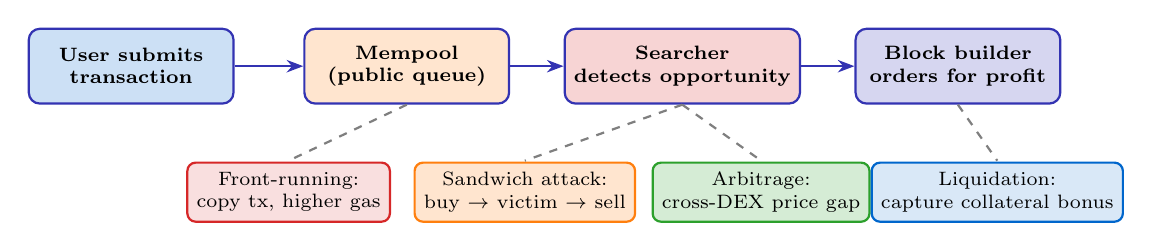
\begin{tikzpicture}[
    box/.style={rectangle, rounded corners=4pt, minimum width=2.6cm, minimum height=0.95cm,
      draw=mlpurple, thick, align=center, font=\scriptsize\bfseries},
    arr/.style={-{Stealth[length=6pt]}, thick, mlpurple}
  ]
    \node[box, fill=mlblue!20]   (usr)  at (0,0)    {User submits\\transaction};
    \node[box, fill=mlorange!20] (mem)  at (3.5,0)  {Mempool\\(public queue)};
    \node[box, fill=mlred!20]    (srch) at (7.0,0)  {Searcher\\detects opportunity};
    \node[box, fill=mlpurple!20] (bld)  at (10.5,0) {Block builder\\orders for profit};

    \draw[arr] (usr.east)  -- (mem.west);
    \draw[arr] (mem.east)  -- (srch.west);
    \draw[arr] (srch.east) -- (bld.west);

    % MEV type labels below
    \node[rectangle, rounded corners=3pt, minimum width=2.5cm, minimum height=0.75cm,
      fill=mlred!15, draw=mlred, thick, align=center, font=\scriptsize]
      (fr) at (2.0,-1.6) {Front-running:\\copy tx, higher gas};
    \node[rectangle, rounded corners=3pt, minimum width=2.5cm, minimum height=0.75cm,
      fill=mlorange!20, draw=mlorange, thick, align=center, font=\scriptsize]
      (sw) at (5.0,-1.6) {Sandwich attack:\\buy $\to$ victim $\to$ sell};
    \node[rectangle, rounded corners=3pt, minimum width=2.5cm, minimum height=0.75cm,
      fill=mlgreen!20, draw=mlgreen, thick, align=center, font=\scriptsize]
      (arb) at (8.0,-1.6) {Arbitrage:\\cross-DEX price gap};
    \node[rectangle, rounded corners=3pt, minimum width=2.5cm, minimum height=0.75cm,
      fill=mlblue!15, draw=mlblue, thick, align=center, font=\scriptsize]
      (liq) at (11.0,-1.6) {Liquidation:\\capture collateral bonus};

    \draw[thick, mlgray, dashed] (mem.south) -- (2.0,-1.2);
    \draw[thick, mlgray, dashed] (srch.south) -- (5.0,-1.2);
    \draw[thick, mlgray, dashed] (srch.south) -- (8.0,-1.2);
    \draw[thick, mlgray, dashed] (bld.south)  -- (11.0,-1.2);
  \end{tikzpicture}
  \end{center}
  \vspace{2mm}
  \begin{block}{Scale of MEV}
    Over \$500M in MEV extracted since Ethereum's genesis.
    \textbf{Flashbots} and \textbf{MEV-Boost} have shifted extraction to off-chain block building,
    reducing on-chain gas wars but concentrating power in block builders.
  \end{block}
  \bottomnote{MEV = value extracted by reordering/inserting/censoring txs; front-run, sandwich, arb, liquidation are main types}
\end{frame}

% Frame 52: DeFi Security Best Practices
\begin{frame}{DeFi Security Best Practices}
  \begin{center}
  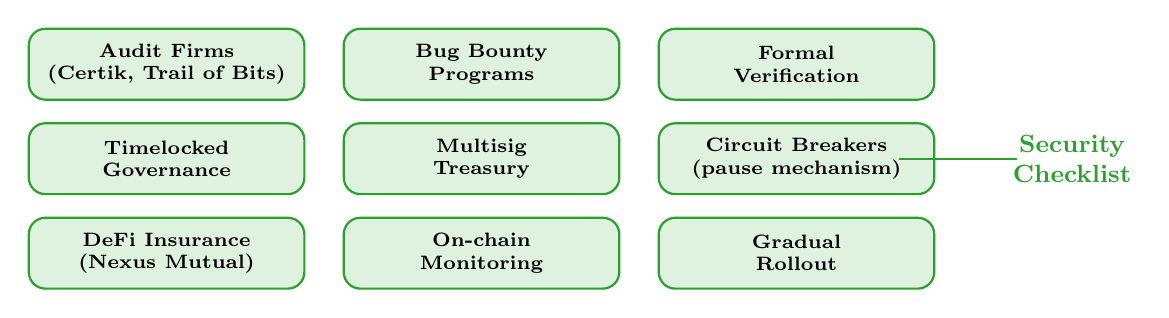
\begin{tikzpicture}[
    shield/.style={rectangle, rounded corners=6pt, minimum width=3.5cm, minimum height=0.9cm,
      draw=mlgreen, thick, fill=mlgreen!15, align=center, font=\scriptsize\bfseries},
    warn/.style={rectangle, rounded corners=6pt, minimum width=3.5cm, minimum height=0.9cm,
      draw=mlorange, thick, fill=mlorange!15, align=center, font=\scriptsize\bfseries}
  ]
    % Row 1
    \node[shield] (a1) at (0,2.6)   {Audit Firms\\(Certik, Trail of Bits)};
    \node[shield] (a2) at (4.0,2.6) {Bug Bounty\\Programs};
    \node[shield] (a3) at (8.0,2.6) {Formal\\Verification};

    % Row 2
    \node[shield] (b1) at (0,1.4)   {Timelocked\\Governance};
    \node[shield] (b2) at (4.0,1.4) {Multisig\\Treasury};
    \node[shield] (b3) at (8.0,1.4) {Circuit Breakers\\(pause mechanism)};

    % Row 3 -- insurance / monitoring
    \node[shield] (c1) at (0,0.2)   {DeFi Insurance\\(Nexus Mutual)};
    \node[shield] (c2) at (4.0,0.2) {On-chain\\Monitoring};
    \node[shield] (c3) at (8.0,0.2) {Gradual\\Rollout};

    % Central shield label
    \node[font=\small\bfseries, text=mlgreen, align=center] at (11.5,1.4) {Security\\Checklist};
    \draw[thick, mlgreen] (9.3,1.4) -- (10.8,1.4);

  \end{tikzpicture}
  \end{center}
  \vspace{1mm}
  \begin{columns}[T]
    \begin{column}{0.48\textwidth}
      \begin{alertblock}{Major Attack Vectors}
        \begin{itemize}\setlength\itemsep{1pt}
          \item Reentrancy (DAO hack, \$60M)
          \item Flash loan oracle manipulation
          \item Access control vulnerabilities
          \item Integer overflow / underflow
        \end{itemize}
      \end{alertblock}
    \end{column}
    \begin{column}{0.48\textwidth}
      \begin{block}{Total DeFi Hacks (cumulative)}
        \textgreater\$7 billion lost to exploits since 2020.
        Audits reduce but do not eliminate risk --- bugs remain
        in audited code.
      \end{block}
    \end{column}
  \end{columns}
  \bottomnote{No audit guarantees safety; defence-in-depth: audits + bug bounties + monitoring + insurance + circuit breakers}
\end{frame}

% Frame 53: Flash Loan Attack Anatomy (TikZ only)
\begin{frame}{Flash Loan Attack Anatomy}
  \begin{center}
  \adjustbox{max width=\textwidth, max totalheight=6.5cm}{%
  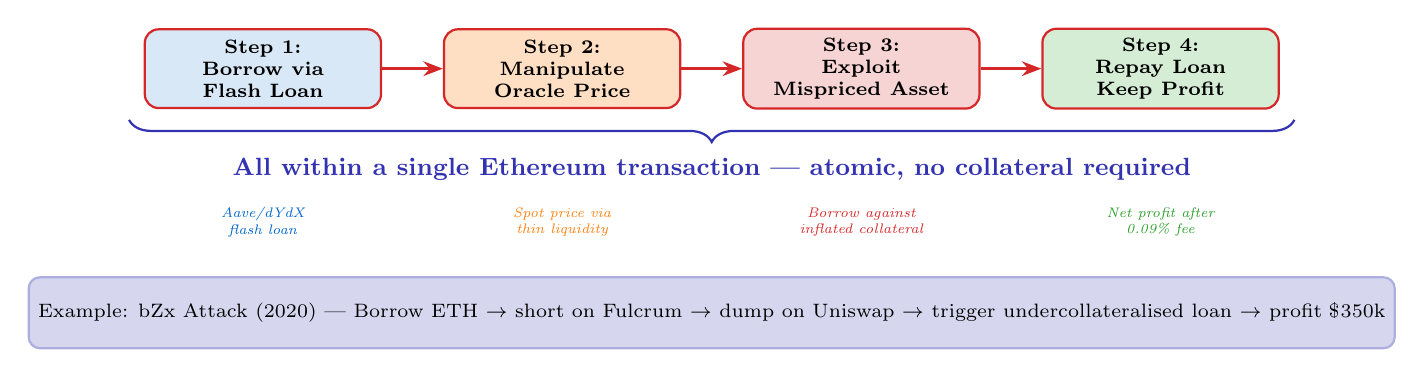
\begin{tikzpicture}[
    atk/.style={rectangle, rounded corners=5pt, minimum width=3.0cm, minimum height=1.0cm,
      draw=mlred, thick, align=center, font=\scriptsize\bfseries},
    arr/.style={-{Stealth[length=7pt]}, very thick, mlred}
  ]
    % Steps in a horizontal flow
    \node[atk, fill=mlblue!15]   (s1) at (0,0)    {Step 1:\\Borrow via\\Flash Loan};
    \node[atk, fill=mlorange!25] (s2) at (3.8,0)  {Step 2:\\Manipulate\\Oracle Price};
    \node[atk, fill=mlred!20]    (s3) at (7.6,0)  {Step 3:\\Exploit\\Mispriced Asset};
    \node[atk, fill=mlgreen!20]  (s4) at (11.4,0) {Step 4:\\Repay Loan\\Keep Profit};

    \draw[arr] (s1.east) -- (s2.west);
    \draw[arr] (s2.east) -- (s3.west);
    \draw[arr] (s3.east) -- (s4.west);

    % Single tx brace
    \draw[thick, mlpurple, decorate, decoration={brace, amplitude=8pt, mirror}]
      (-1.7,-0.65) -- (13.1,-0.65)
      node[midway, below=10pt, font=\small\bfseries, text=mlpurple] {All within a single Ethereum transaction --- atomic, no collateral required};

    % Annotation nodes
    \node[font=\tiny\itshape, text=mlblue, align=center]   at (0,-1.95)   {Aave/dYdX\\flash loan};
    \node[font=\tiny\itshape, text=mlorange, align=center] at (3.8,-1.95) {Spot price via\\thin liquidity};
    \node[font=\tiny\itshape, text=mlred, align=center]    at (7.6,-1.95) {Borrow against\\inflated collateral};
    \node[font=\tiny\itshape, text=mlgreen, align=center]  at (11.4,-1.95){Net profit after\\0.09\% fee};

    % Example
    \node[rectangle, rounded corners=4pt, minimum width=13.5cm, minimum height=0.9cm,
      fill=mllavender4, draw=mllavender, thick, align=center, font=\scriptsize]
      at (5.7,-3.1)
      {Example: bZx Attack (2020) --- Borrow ETH $\to$ short on Fulcrum $\to$ dump on Uniswap $\to$
       trigger undercollateralised loan $\to$ profit \$350k};
  \end{tikzpicture}
  }%
  \end{center}
  \bottomnote{Flash loan attacks exploit atomic composability; defence: TWAP oracles, circuit breakers, reentrancy guards}
\end{frame}

% Frame 54: DeFi Regulation Landscape
\begin{frame}{DeFi Regulation Landscape}
  \begin{center}
  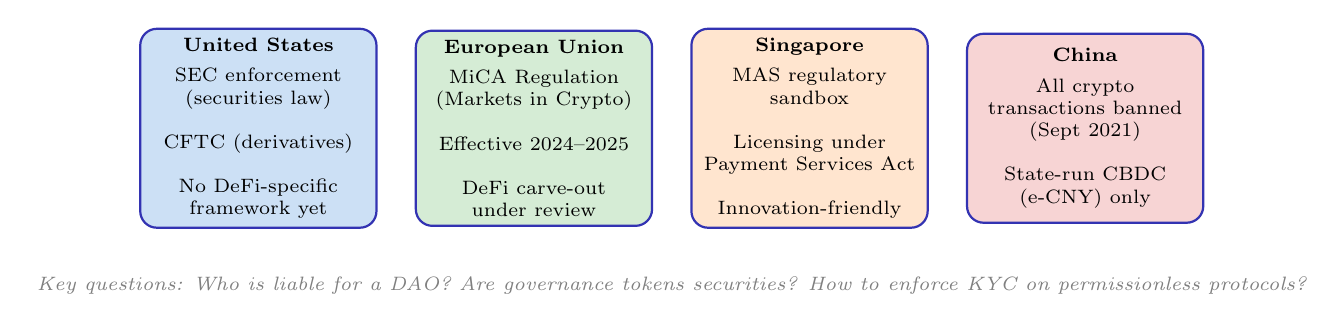
\begin{tikzpicture}[
    regbox/.style={rectangle, rounded corners=6pt, minimum width=3.0cm, minimum height=2.4cm,
      draw=mlpurple, thick, align=center, font=\scriptsize}
  ]
    % Region boxes
    \node[regbox, fill=mlblue!20]   (us)  at (0,0)    {\textbf{United States}\\[3pt]
      SEC enforcement\\(securities law)\\\\
      CFTC (derivatives)\\\\
      No DeFi-specific\\framework yet};

    \node[regbox, fill=mlgreen!20]  (eu)  at (3.5,0)  {\textbf{European Union}\\[3pt]
      MiCA Regulation\\(Markets in Crypto)\\\\
      Effective 2024--2025\\\\
      DeFi carve-out\\under review};

    \node[regbox, fill=mlorange!20] (sg)  at (7.0,0)  {\textbf{Singapore}\\[3pt]
      MAS regulatory\\sandbox\\\\
      Licensing under\\Payment Services Act\\\\
      Innovation-friendly};

    \node[regbox, fill=mlred!20]    (cn)  at (10.5,0) {\textbf{China}\\[3pt]
      All crypto\\transactions banned\\(Sept 2021)\\\\
      State-run CBDC\\(e-CNY) only};

    % Question labels below
    \node[font=\scriptsize\itshape, text=mlgray, align=center] at (5.25,-2.0)
      {Key questions: Who is liable for a DAO? Are governance tokens securities?
       How to enforce KYC on permissionless protocols?};
  \end{tikzpicture}
  \end{center}
  \vspace{1mm}
  \begin{block}{Regulatory Trajectory}
    Most jurisdictions are moving toward \textbf{activity-based regulation} (what you do, not what
    technology you use). Centralised interfaces (front-ends) are increasingly targeted, even
    when underlying smart contracts remain permissionless.
  \end{block}
  \bottomnote{Regulation varies: US (enforcement), EU (MiCA), Singapore (sandbox), China (banned); DAO liability unresolved}
\end{frame}

% Frame 55: Key Takeaways and Course Summary
\begin{frame}{Key Takeaways and Course Summary}
  \vspace{1mm}
  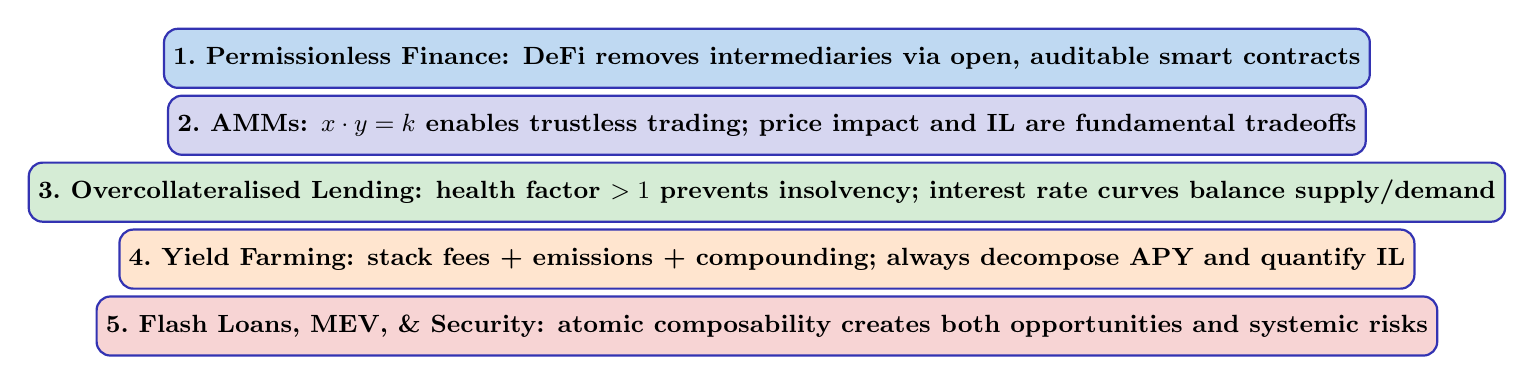
\begin{tikzpicture}[
    tkbox/.style={rectangle, rounded corners=5pt, minimum width=13.5cm, minimum height=0.75cm,
      draw=mlpurple, thick, align=center, font=\small\bfseries}
  ]
    \node[tkbox, fill=mlblue!25]    (t1) at (0,0)    {%
      1.\ Permissionless Finance: DeFi removes intermediaries via open, auditable smart contracts};
    \node[tkbox, fill=mlpurple!20]  (t2) at (0,-0.85) {%
      2.\ AMMs: $x \cdot y = k$ enables trustless trading; price impact and IL are fundamental tradeoffs};
    \node[tkbox, fill=mlgreen!20]   (t3) at (0,-1.70) {%
      3.\ Overcollateralised Lending: health factor $>1$ prevents insolvency; interest rate curves balance supply/demand};
    \node[tkbox, fill=mlorange!20]  (t4) at (0,-2.55) {%
      4.\ Yield Farming: stack fees + emissions + compounding; always decompose APY and quantify IL};
    \node[tkbox, fill=mlred!20]     (t5) at (0,-3.40) {%
      5.\ Flash Loans, MEV, \& Security: atomic composability creates both opportunities and systemic risks};
  \end{tikzpicture}

  \vspace{2mm}
  \begin{beamercolorbox}[sep=6pt,center,rounded=true,shadow=true]{palette quaternary}
    {\bfseries Course Complete --- DeFi Fundamentals: A Quantitative Deep Dive}\\[2pt]
    {\small 5 Sections $|$ 55 Frames $|$ Prof.\ Dr.\ Joerg Osterrieder}
  \end{beamercolorbox}
  \bottomnote{Course complete | All 5 sections delivered | Continue with Lesson 6: DeFi Risk Management}
\end{frame}

\end{document}
